\chapter{Discussion}
\section{Data Analysis of Study}
As discussed, the participants had to fill out a small questionnaire every day in the evening and these answers were then matched against the computed results. The study resulted in a dataset with 205 days of data, corresponding to 2.51M timestamped location data points, spread over 10 participants. Table \ref{tab:location-samples} shows the overview of the data collected for each participant, including the number of points, number of days and the storage requirements for the collected data.\\

Similar to Cuttone et al. \cite{sparse-location-2014}, the participants have been anonymized as \textit{P1} through \textit{P9}, and the author has been marked as \textit{R} (researcher).\\

\begin{table}[]
    \centering
        \begin{tabular}{|l|l|l|l|l|l|}
        \hline
        {\ul \textbf{P}} & {\ul \textbf{Days}} & {\ul \textbf{Samples}} & {\ul \textbf{MB}} & {\ul \textbf{Samples/day}} & {\ul \textbf{MB/day}} \\ \hline
        \textbf{P1}                & 23                   & 181                        & 17.3                           & 7878.8                              & 0.8                              \\ \hline
        \textbf{P2}                & 25                   & 142                        & 13.6                           & 5684.4                              & 0.5                             \\ \hline
        \textbf{P3}                & 21                   & 101                        & 9.7                            & 4850.7                              & 0.5                             \\ \hline
        \textbf{P4}                & 22                   & 98                         & 9.4                            & 4494.9                              & 0.4                             \\ \hline
        \textbf{P5}                & 14                   & 209                        & 20.0                           & 14977.4                             & 1.4                             \\ \hline
        \textbf{P6}                & 26                   & 101                        & 9.7                            & 3922.8                              & 0.4                             \\ \hline
        \textbf{P7}                & 23                   & 111                       & 106.4                          & 48525.0                             & 4.6                             \\ \hline
        \textbf{P8}                & 15                   & 141                        & 13.5                           & 9417.3                              & 0.9                              \\ \hline
        \textbf{P9}                & 12                   & 51                         & 4.9                            & 4311.7                              & 0.4                              \\ \hline
        \textbf{R}                 & 24                   & 365                        & 34.9                           & 15233.6                             & 1.5                                    \\ \hline
        \end{tabular}

    \caption{The overview of collected Location Samples for each participant in the study}
    \label{tab:location-samples}
\end{table}

The answers were of a different format than the computed features and therefore had to be converted into scalars such that they could be compared directly to the features. For the Home Stay feature, the answer the users gave was the number of hours away from home, at the time of registering. It was assumed that most people be registering at home since the diary was filled out in the evening. Therefore for calculating the Home Stay value from a given answer $a$, equation \ref{eq:home-stay-ans} was applied:

\begin{equation}
\label{eq:home-stay-ans}
    h = \frac{t - a }{t}
\end{equation}

Here, $t$ refers to the timestamp at which the diary was filled out.

For the \textit{Routine Index}, the answer (a number of 0 to 5) was transformed to scalar between 0 and 1, i.e. let the scale value be $s \in \{0, 1, 2, 3, 4, 5\}$, then the corresponding \textit{Routine Index} is calculated using equation \ref{eq:routine-ans}.

\begin{equation}
\label{eq:routine-ans}
    r = \frac{s}{s_{max}}, \quad s_{max} = 5
\end{equation}

Regarding data collection, figure \ref{fig:plot-num-points-stops} displays how much data was collected per participant. From this figure, it is clear that some participants did not collect nearly as much data as others, and because of this their computed features are expected to be more inaccurate. It was also discovered that the number of stops found is not necessarily correlated with the number of location samples found, as can be seen for participant P7. This can be due to reasons such as moving around much less, which results in fewer but stops with a longer duration being found. \\

\begin{figure}
    \centering
    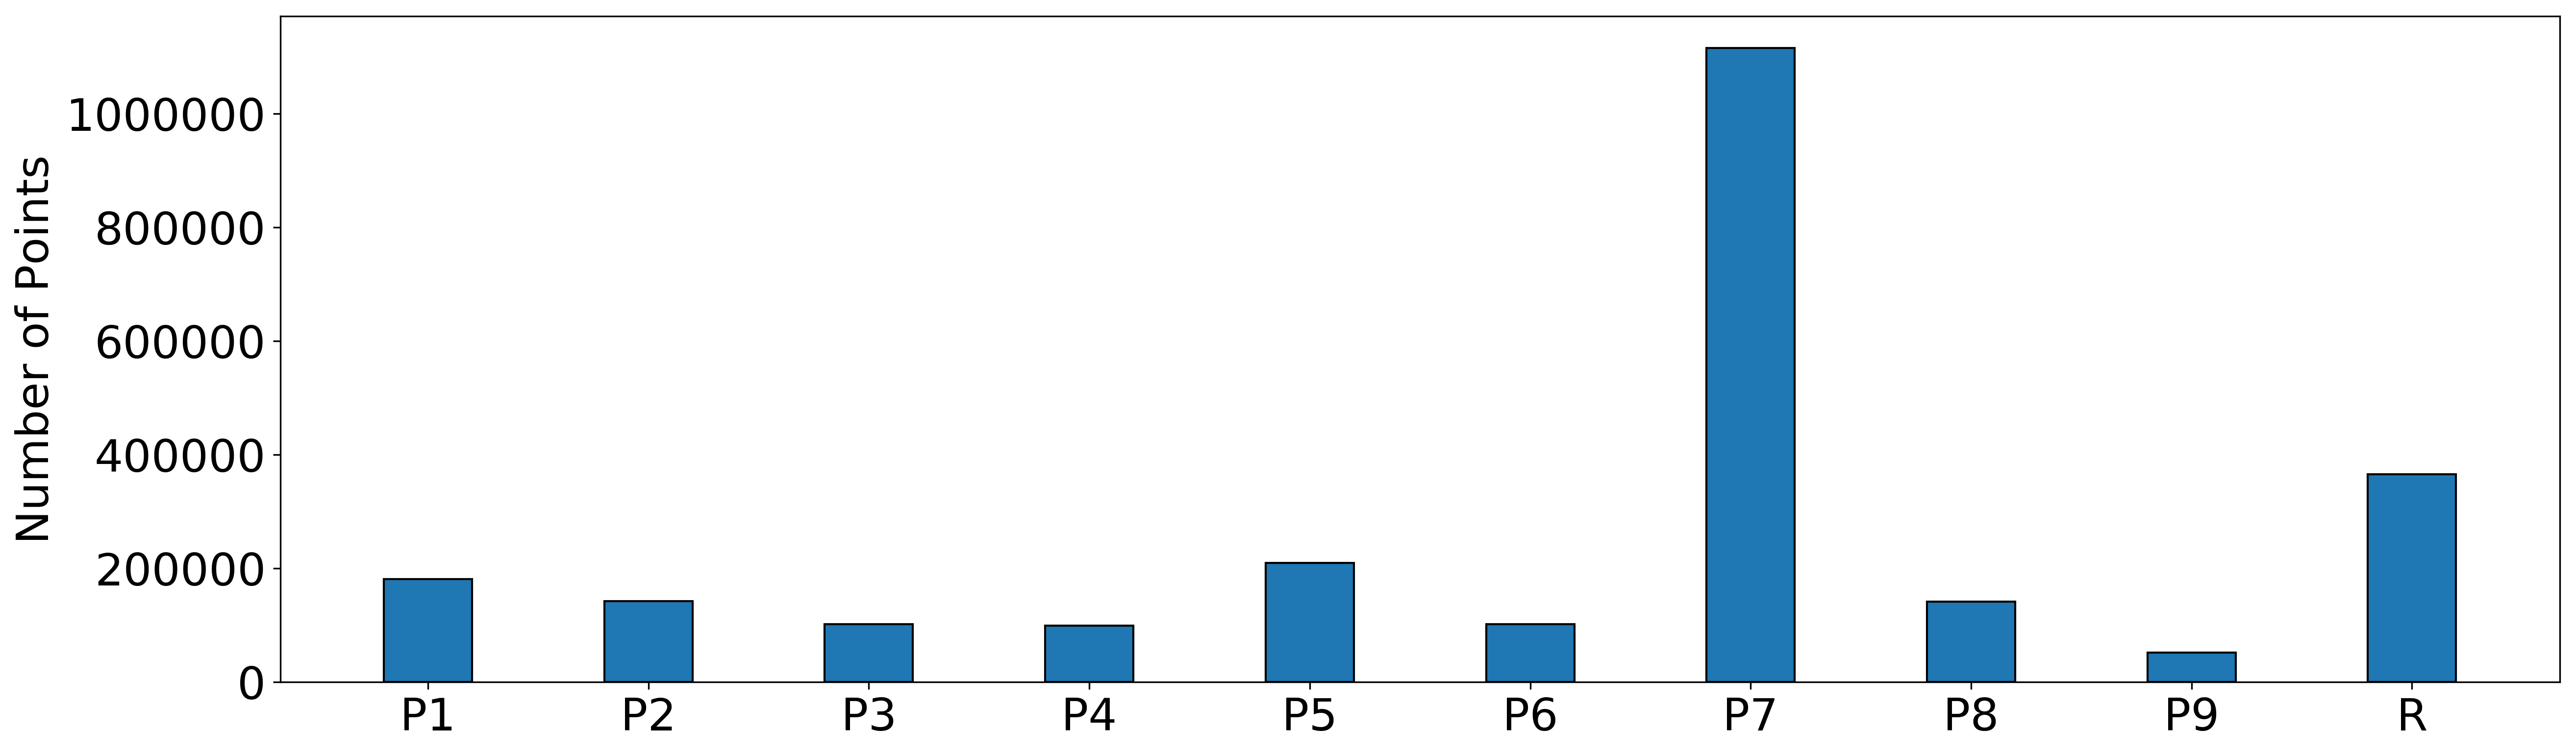
\includegraphics[width=\textwidth]{images/study/storage/num_points.png}
    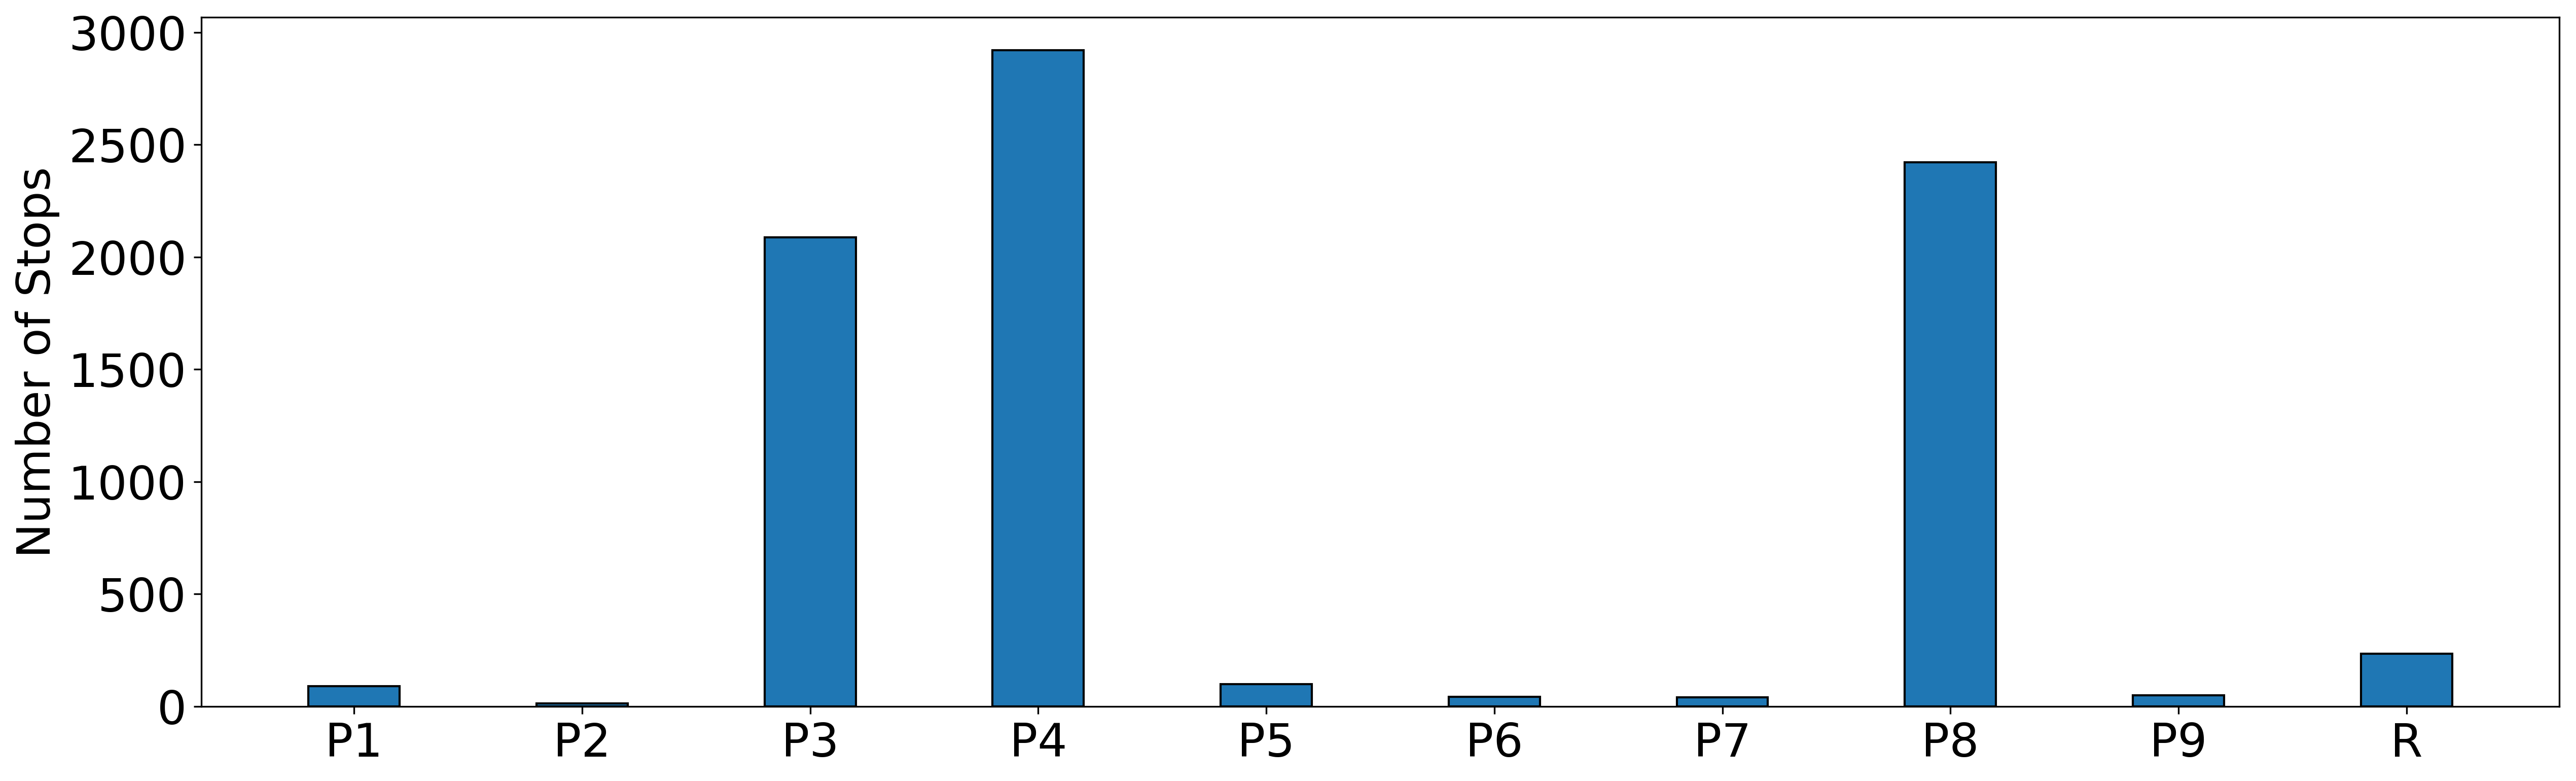
\includegraphics[width=\textwidth]{images/study/storage/num_stops.png}
    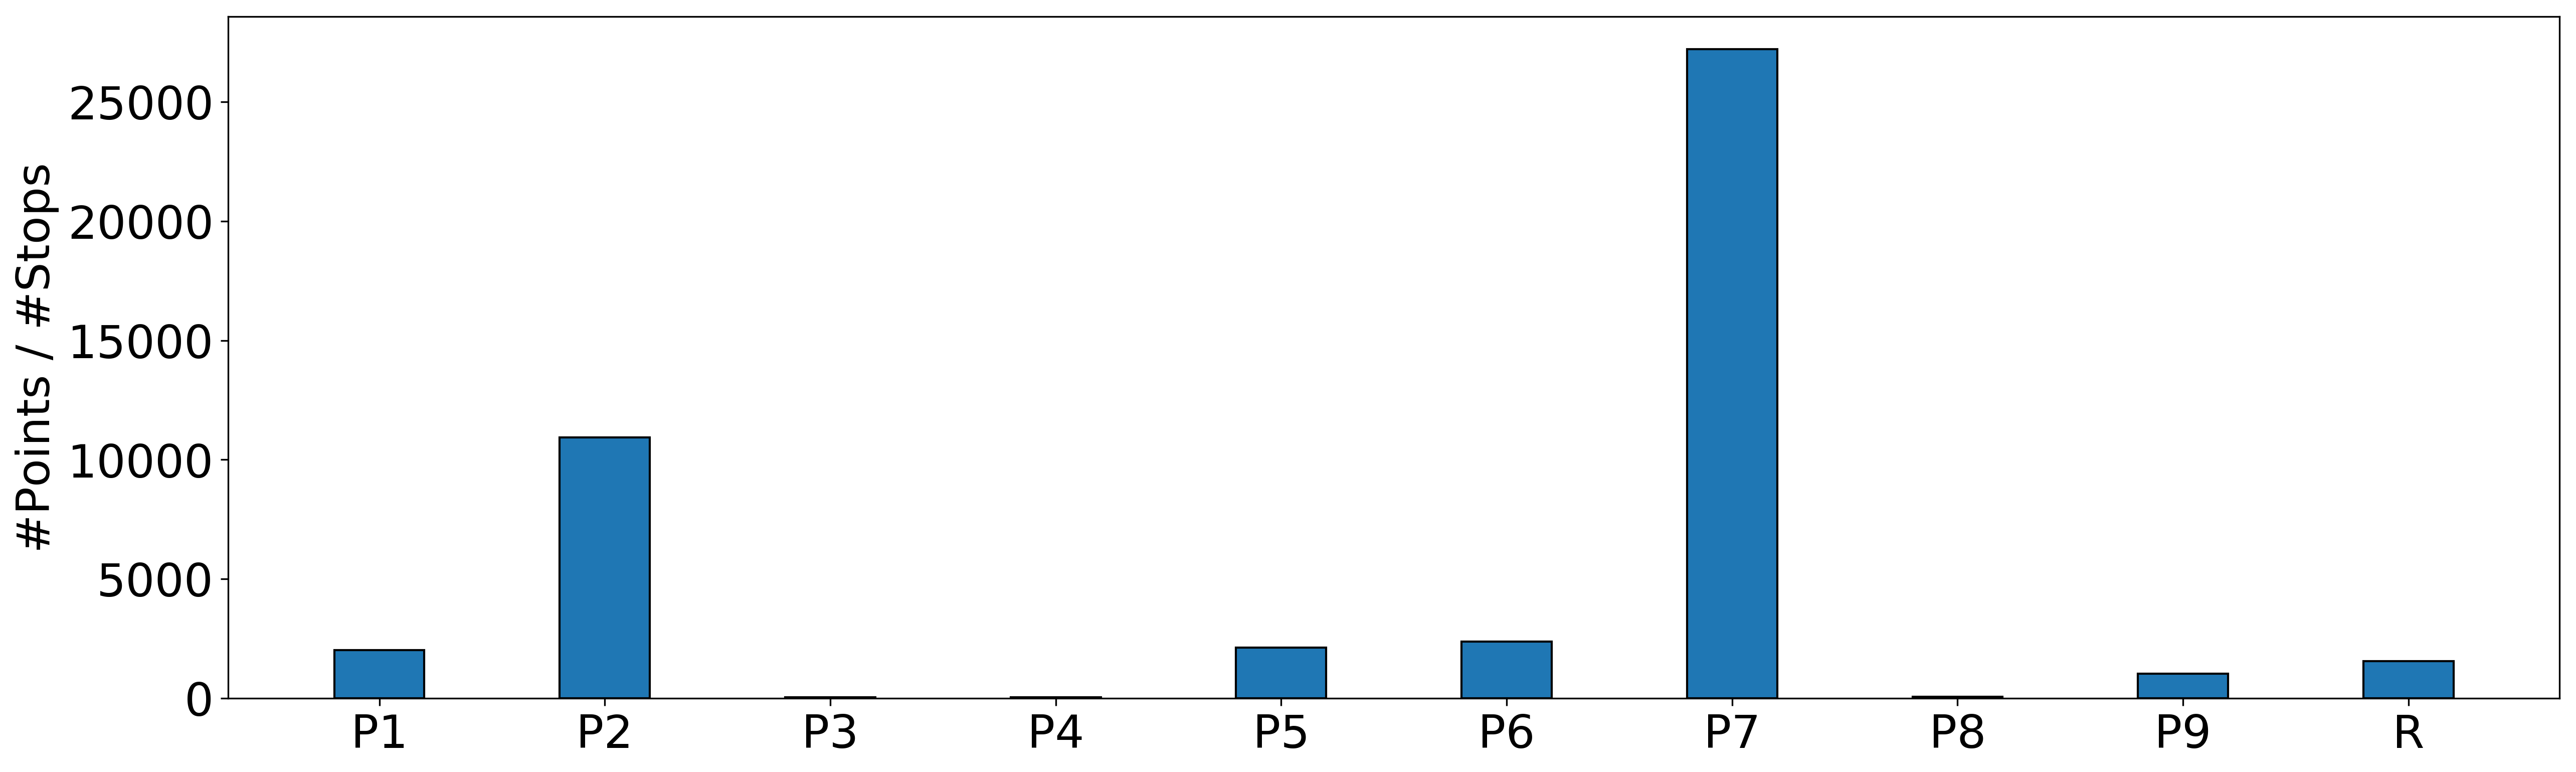
\includegraphics[width=\textwidth]{images/study/storage/compression_N.png}
    \caption{The number of raw location samples (top) and the number of stops (middle) collected, and the ratio between the two, for each participant}
    \label{fig:plot-num-points-stops}
\end{figure}

\begin{figure}
    \centering
    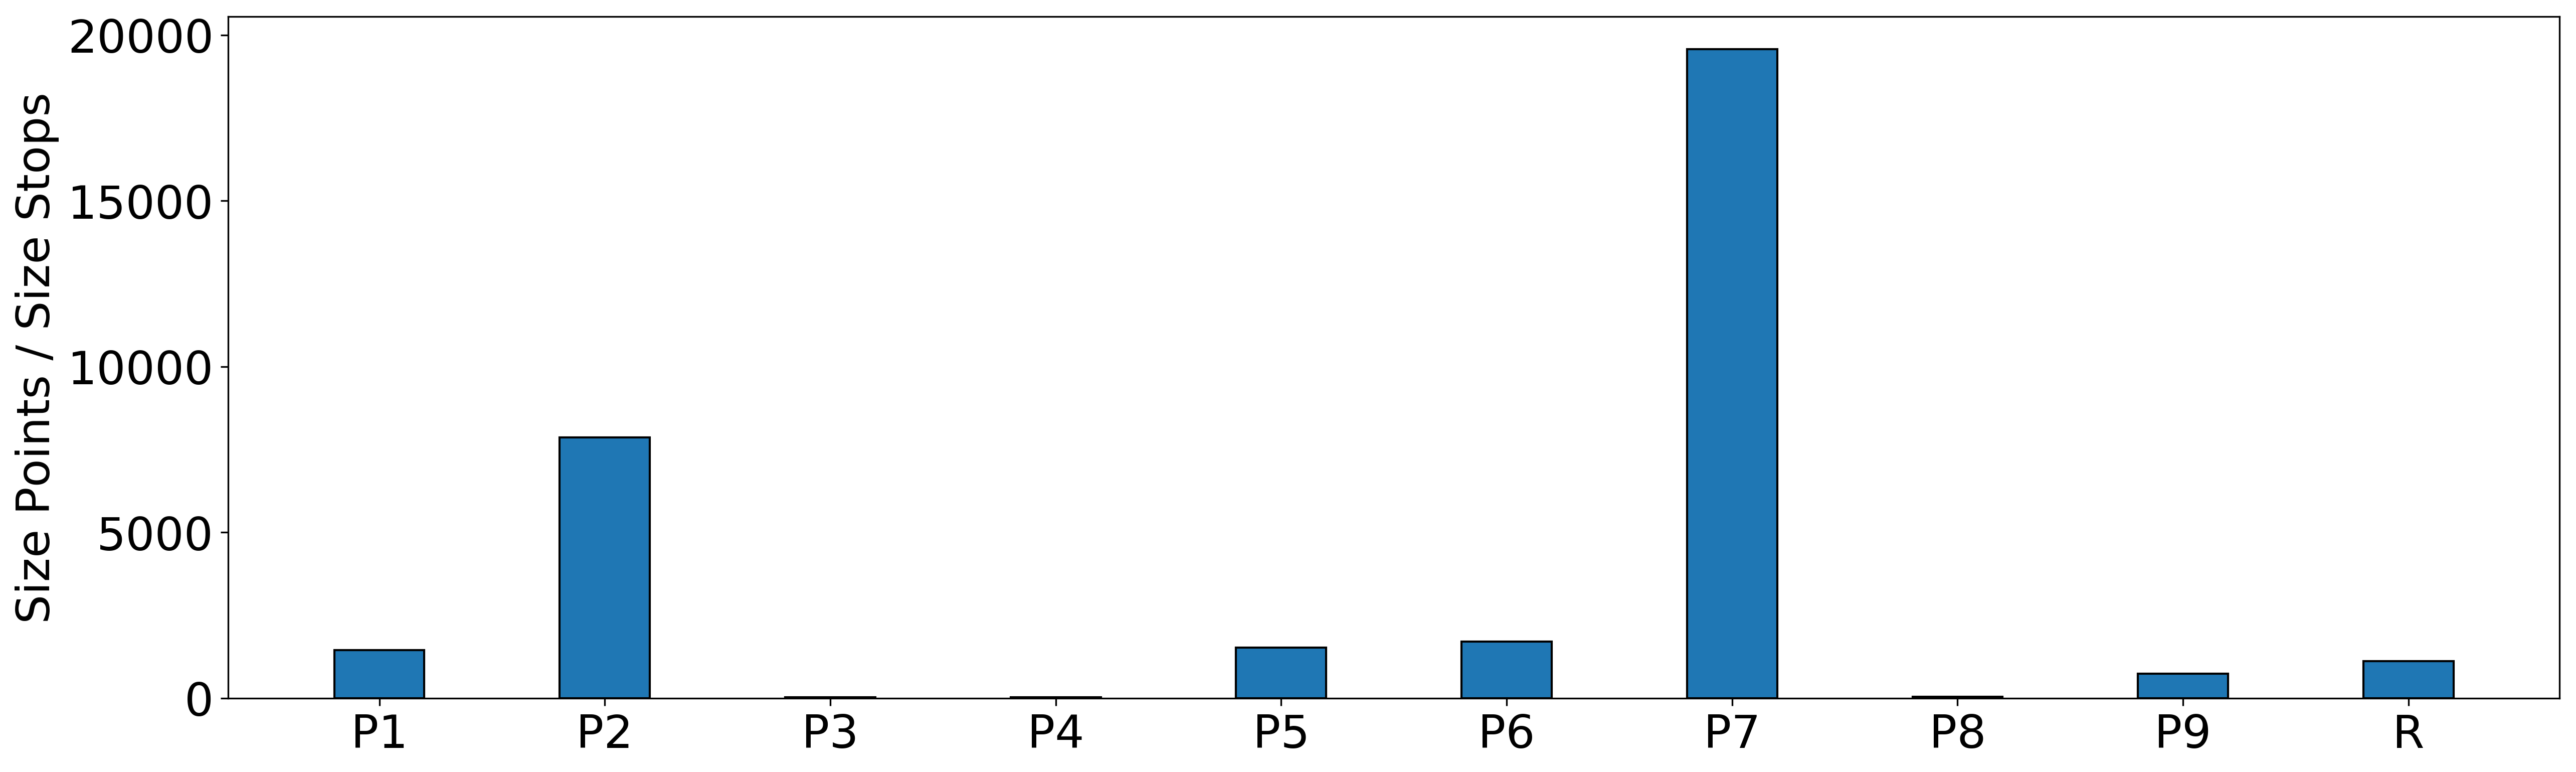
\includegraphics[width=\textwidth]{images/study/storage/compression_mb.png}
    \caption{The ratio between location samples and stops expressed in terms of storage, in MB}
    \label{fig:plot-num-points-stops}
\end{figure}

The average size of a serialized \textit{LocationSample} was compted based on file size to be around 100 bytes, with a stop is being 140 bytes. With this information, it is possible to calculate the compression rate for each participant, i.e. how much their dataset was reduced by converting location samples into stops, and this is shown in Figure \ref{fig:plot-num-points-stops}. The number of valid days for a specific feature is the number of days for which the user gave answers, and the feature could be calculated. If the user for example turned off their phone during the night, the Home Stay feature could not be calculated, but the routine index feature and the number of places will likely still have been calculated.

\subsection{Subjectivity of Answers and Ground Truth}
A thing to keep in mind is that the participants' answers are not ground truth, and there are multiple reasons why a participant's answer may be inaccurate. Firstly, people's subjective recollection is not necessarily as accurate as they think it might me. Secondly, it was not communicated explicitly to the participants what exactly counts as a place, and how their 'routine' is calculated - this means that participants may have filled out the questionnaire differently, given the same ground truth data - for example, whether or not being in the garden counts as being home. Thirdly, some users misunderstood the routine scale, and users whose data looked strange were contacted afterward to enquire about whether they had misunderstood the question, and if so the answers were corrected as much as could be done. Lastly, the hour away from home and routine index answers were very course-grained, and therefore the participants were probably rarely able to give exact answers, according to their own recollection. 

\subsection{Missing Location Data and Answers}
The sampling was set to once per second, yet data was not sampled uniformly. In fact, there were many gaps in the collected data. Figure \ref{fig:plot-gaps-data} shows the data of the author collected during the study over 24 days. The author was very diligent in tracking his location and yet substantial gaps in the data can be observed. These gaps are consistent in the morning where the phone is not moving around, but after 6 AM it seems there is no pattern for the gaps. The event plot for the collected data for particpant P8 is shown  in Figre \ref{fig:p8-gaps} in Appendix \ref{appendix:data-analysis}. \\


\begin{figure}[h]
    \centering
    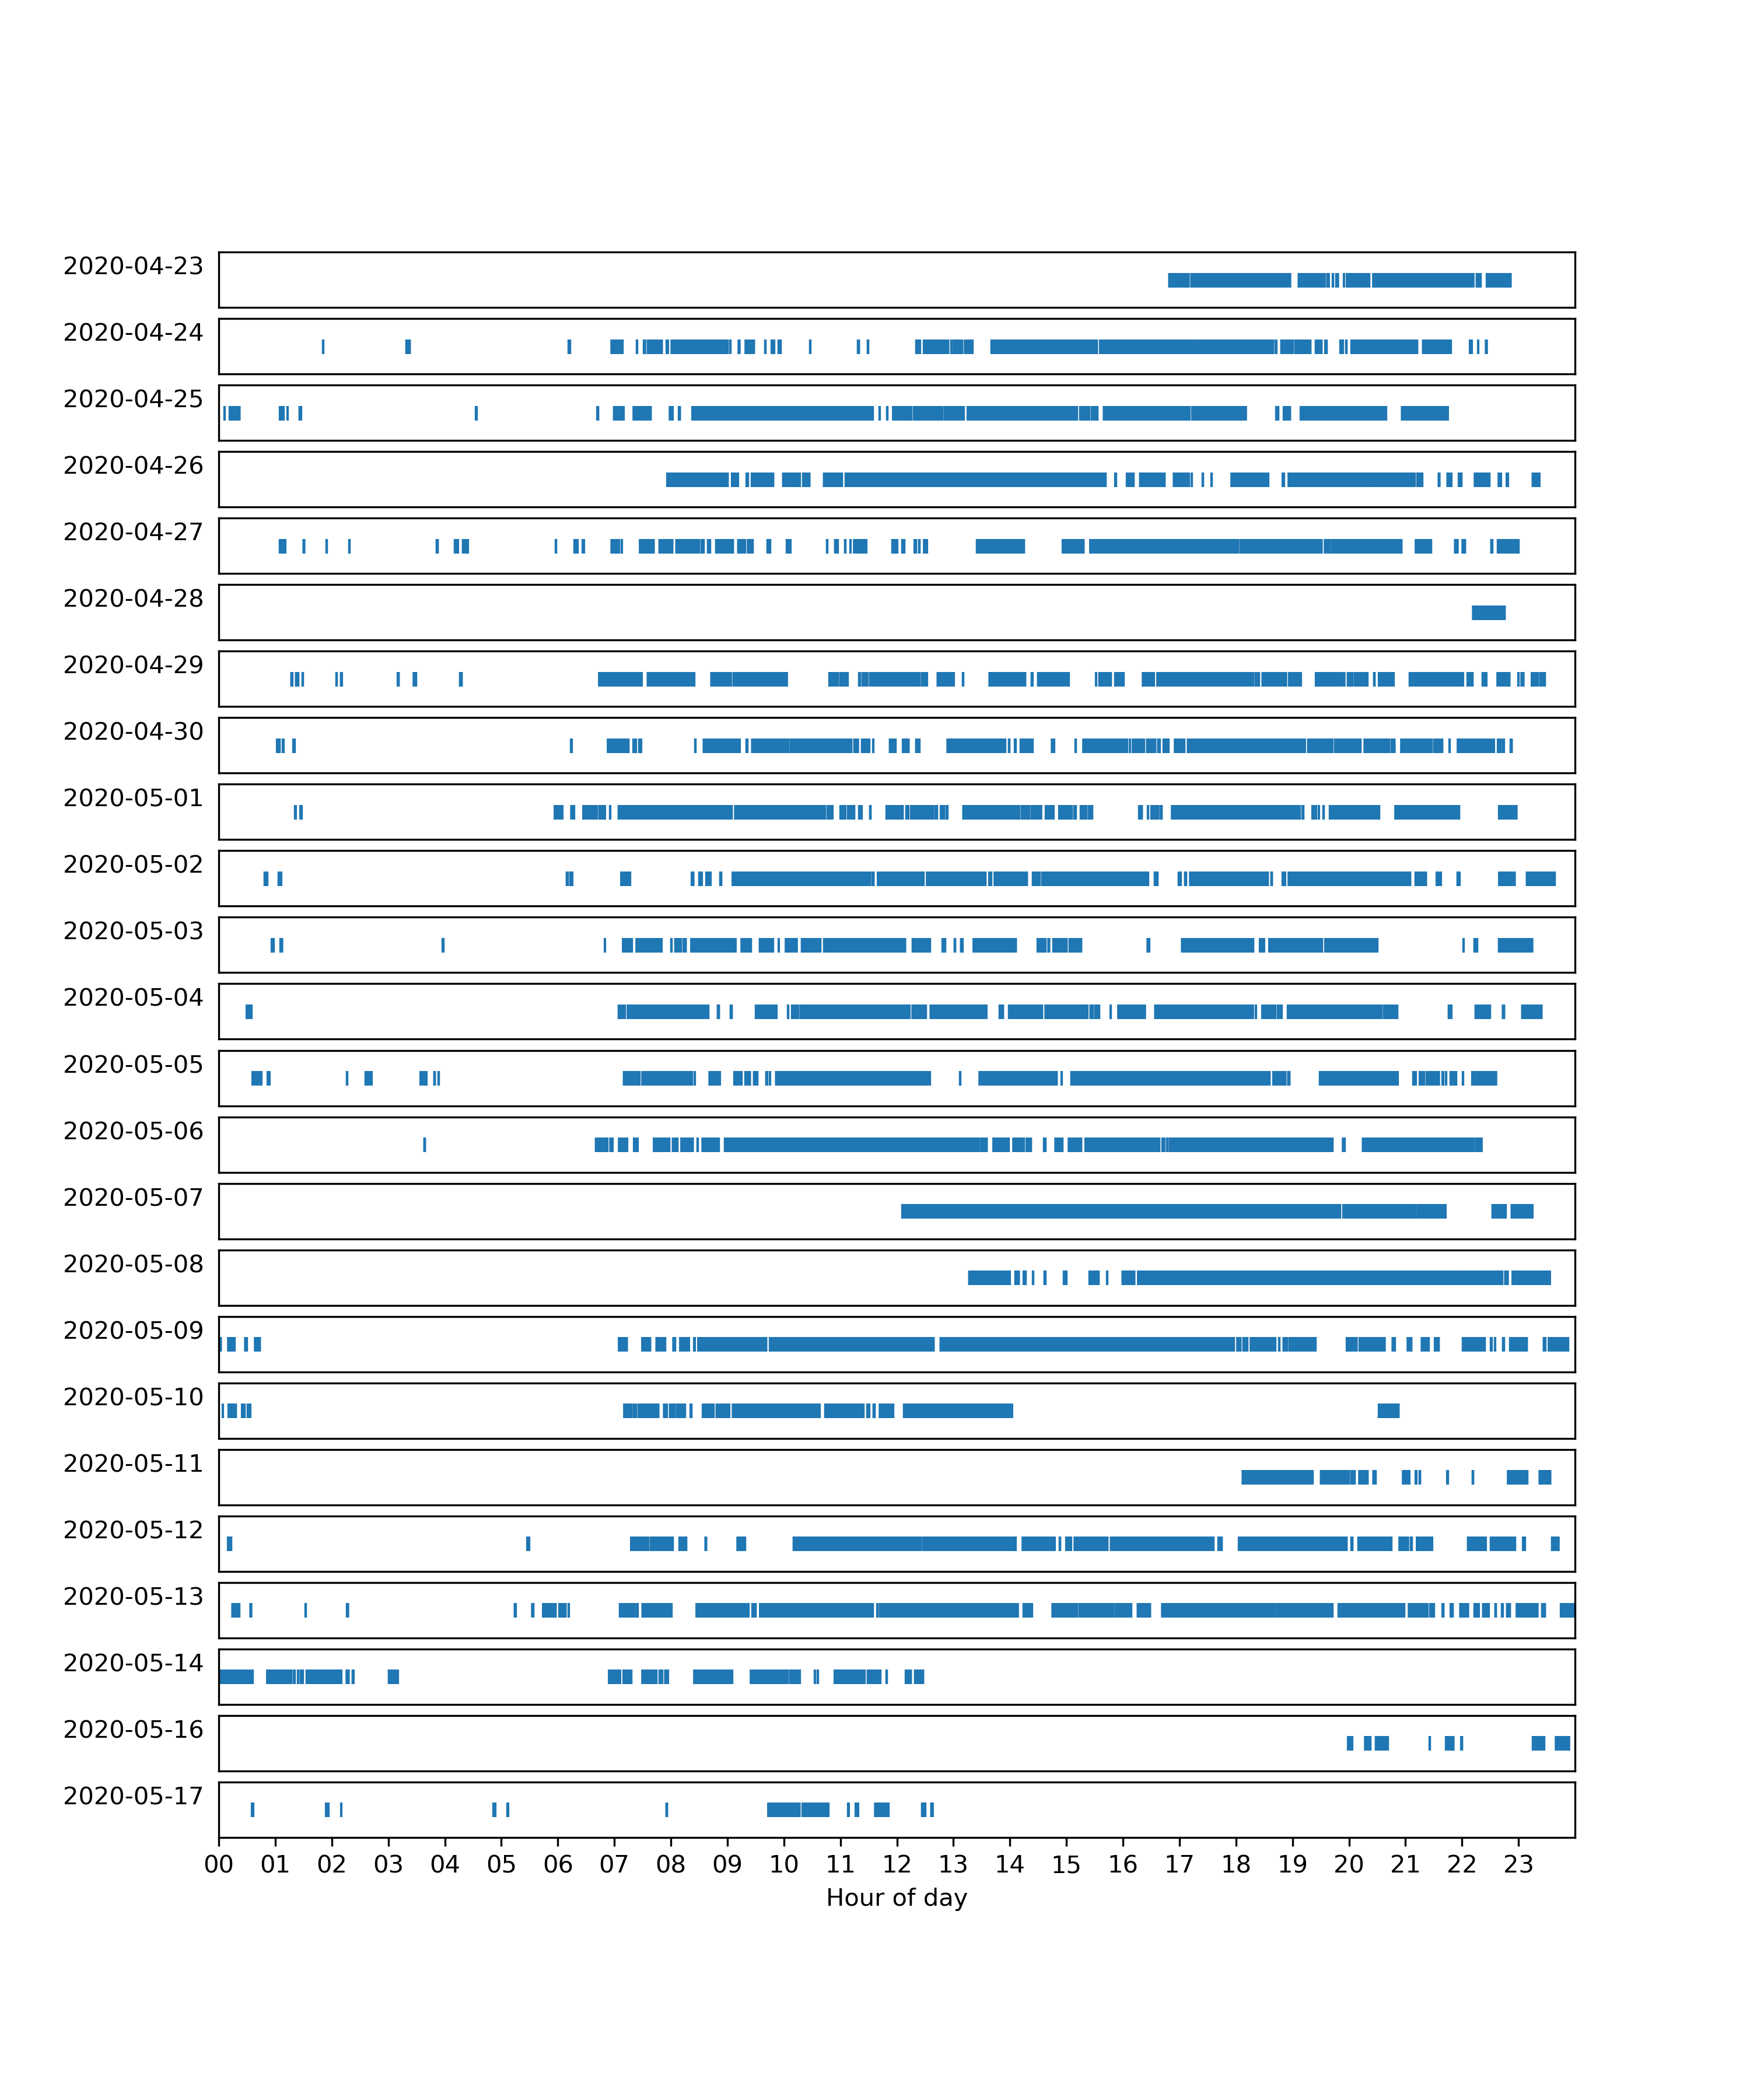
\includegraphics[width=\textwidth]{images/study/thomas-gaps.png}
    \caption{An event plot for the author's sampled location data, each day of the study. As can be seen there are quite a few gaps in the data which will make the computes features less accurate}
    \label{fig:plot-gaps-data}
\end{figure}

Regarding the subjective user data, many users missed filling out the diary on several days. Figure \ref{fig:plot-days-answered} shows the number of total days where a participant participated in the study against the days on which they provided an answer. It was only possible to calculate the error between computed features and the answers on day, if the participant gave an answer. This means that for some participants, a lot of data was thrown away for the data analysis. As an example, it was considered whether or not to entirely get rid of P9 since he/she has very little data both terms of total days collected and even fewer in terms of days with answers. 

\begin{figure}[h]
    \centering
    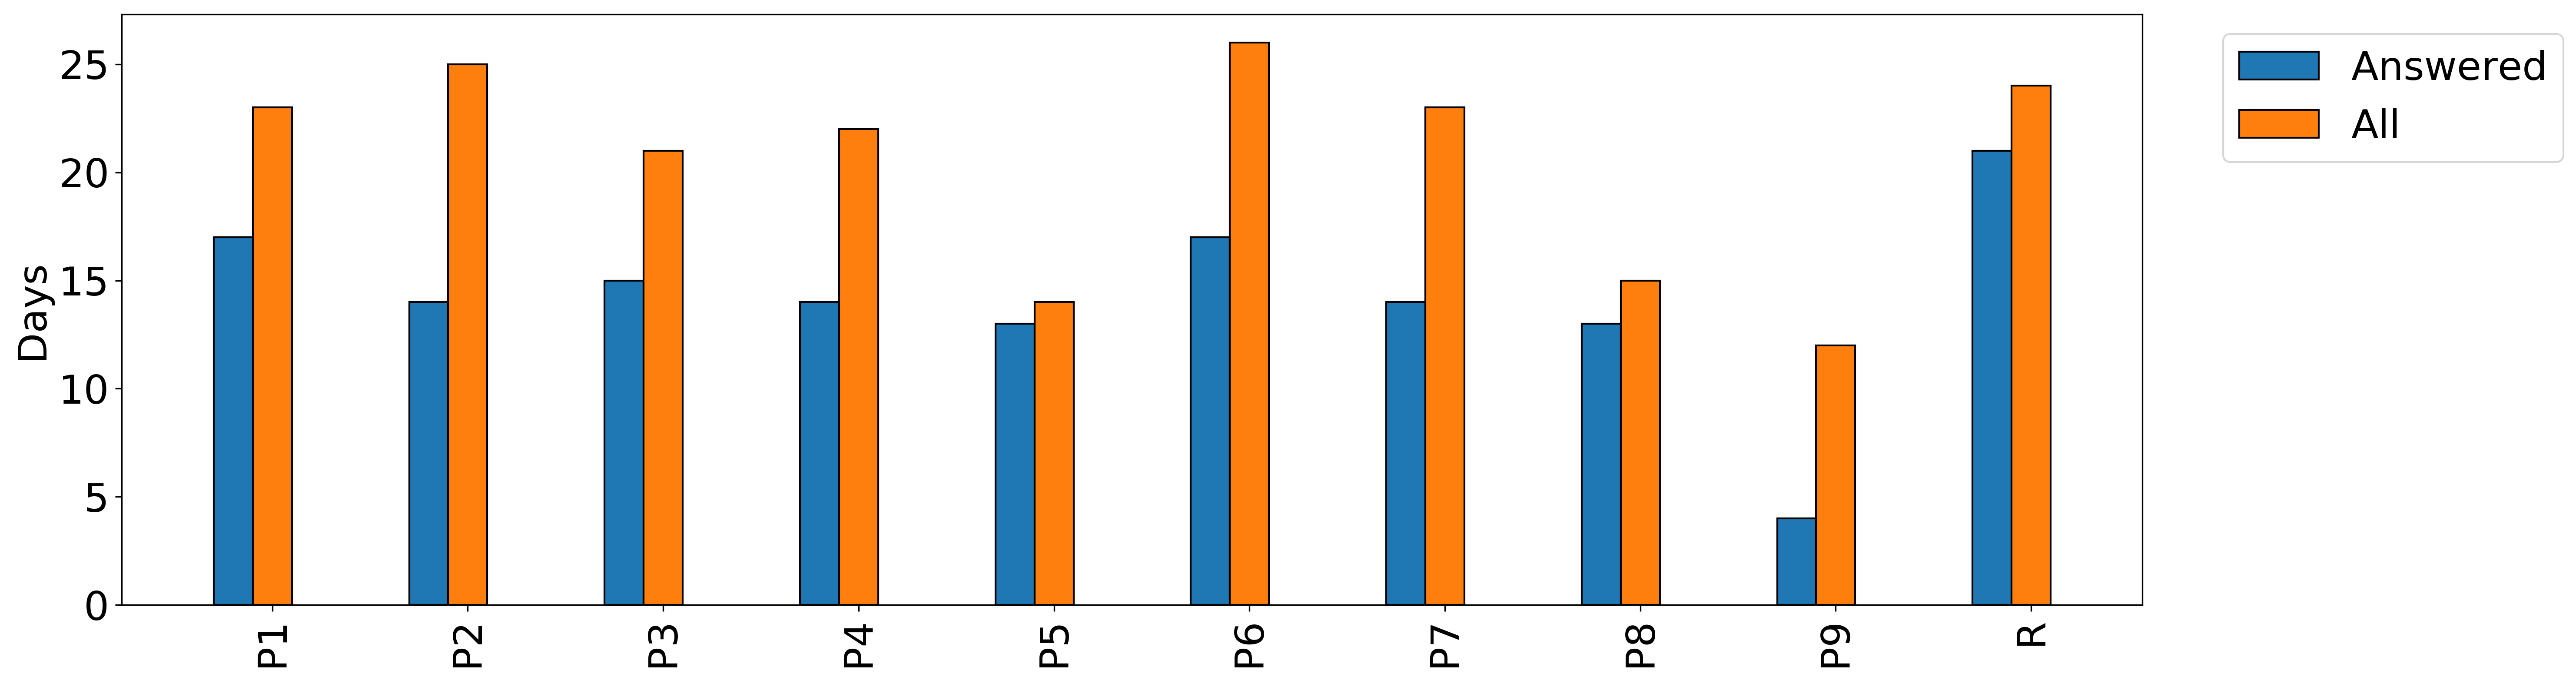
\includegraphics[width=\textwidth]{images/study/storage/answers_days_plot.png}
    \caption{The total number of days of participation vs the days for which the diary was filled out by the participant. As can be seen, some users often forgot to give an answer}
    \label{fig:plot-days-answered}
\end{figure}

Another problem that was encountered was when participants would fill out the questionnaire during the night, or the very next morning due to forgetting the previous evening. This meant the answer for day $n$ would be listed as date $n+1$, i.e. the wrong date. This was rectified by changing all answers given between 00:00 and 10:00 to the previous date at 23:59:59. In addition, some users entirely forgot certain days but remembered it the following day, and reported it manually to the researcher, and these answers were then added manually. 

\subsection{Feature Evaluation}
The Home Stay feature required the participant to track their location during the night, as previously mentioned. This meant that if they did not, the Home Stay feature could not be evaluated for that particular day, however other features might still be available for computation, such as the Number of Places. This meant that the number of days for which a given feature can be compared to the answers is not necessarily the same for all features. 

\begin{figure}[h]
    \centering
    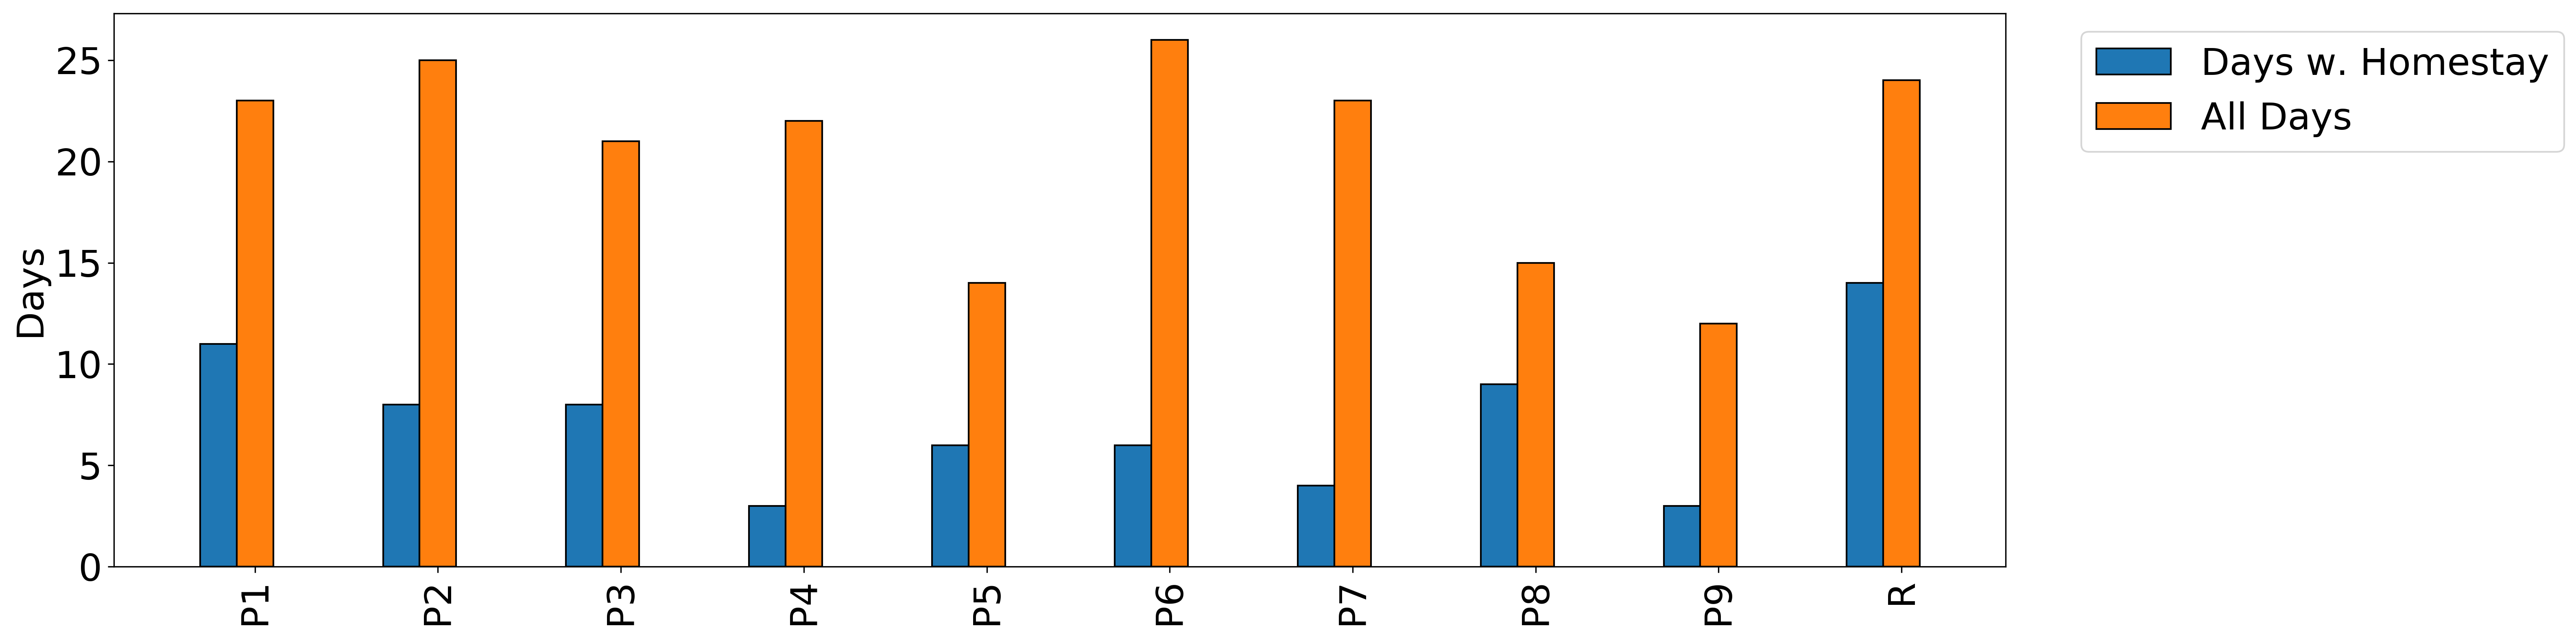
\includegraphics[width=\textwidth]{images/study/homestay_valid_days.png}
    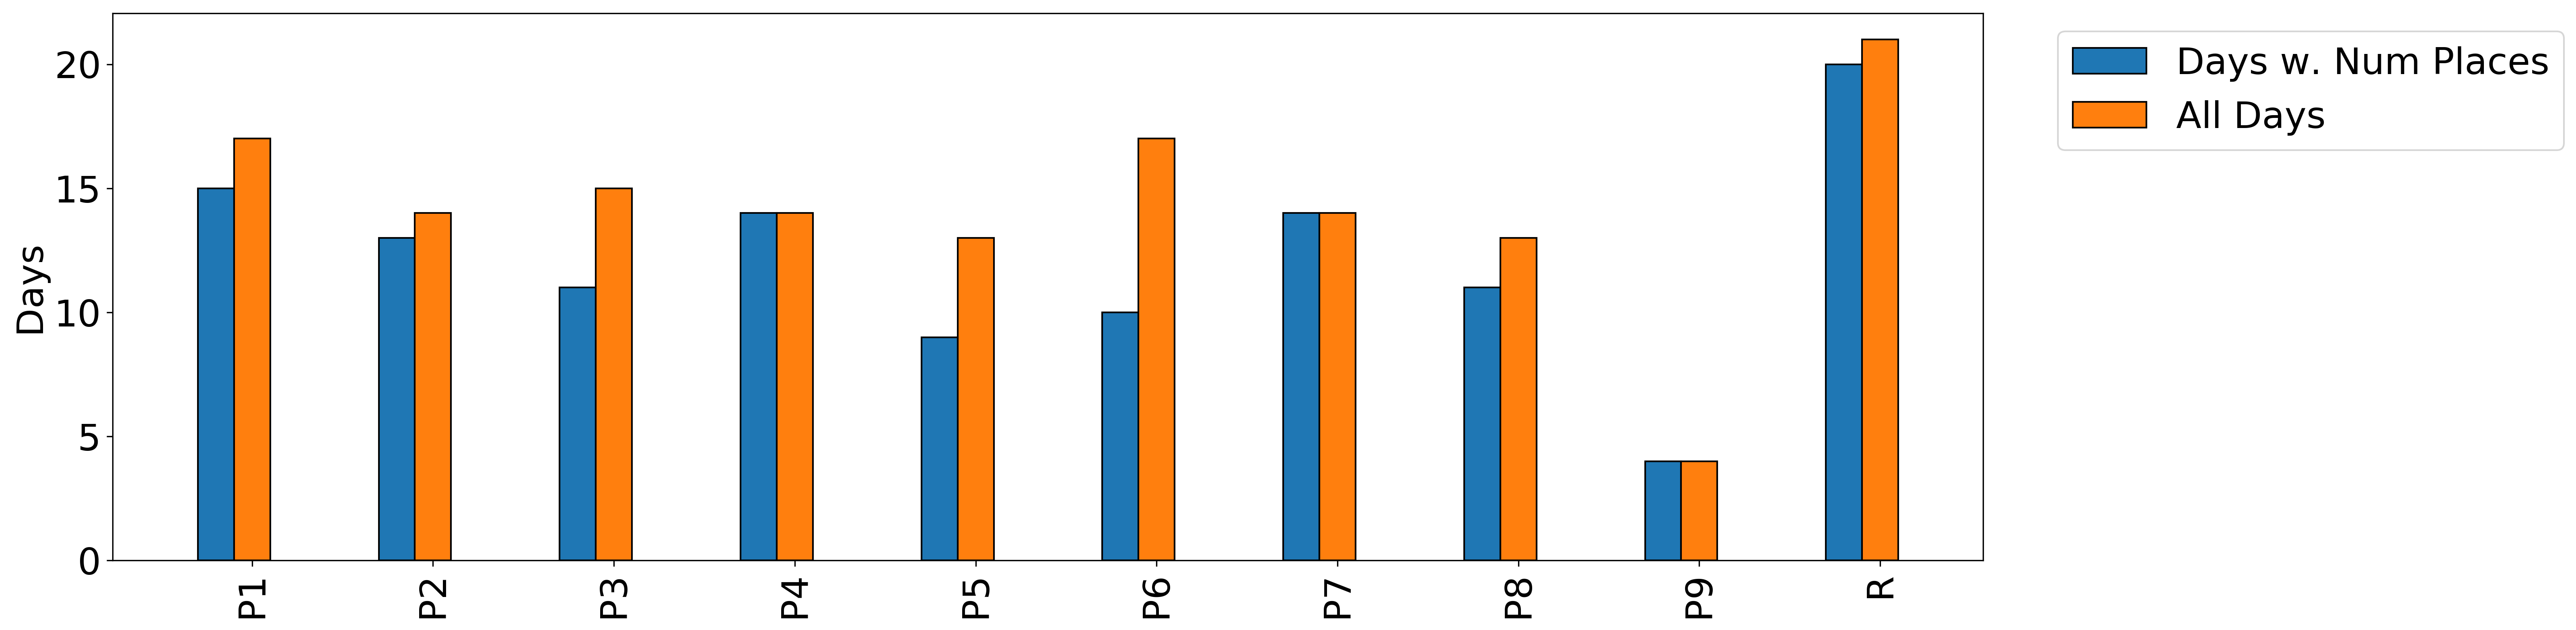
\includegraphics[width=\textwidth]{images/study/numplaces_valid_days.png}
    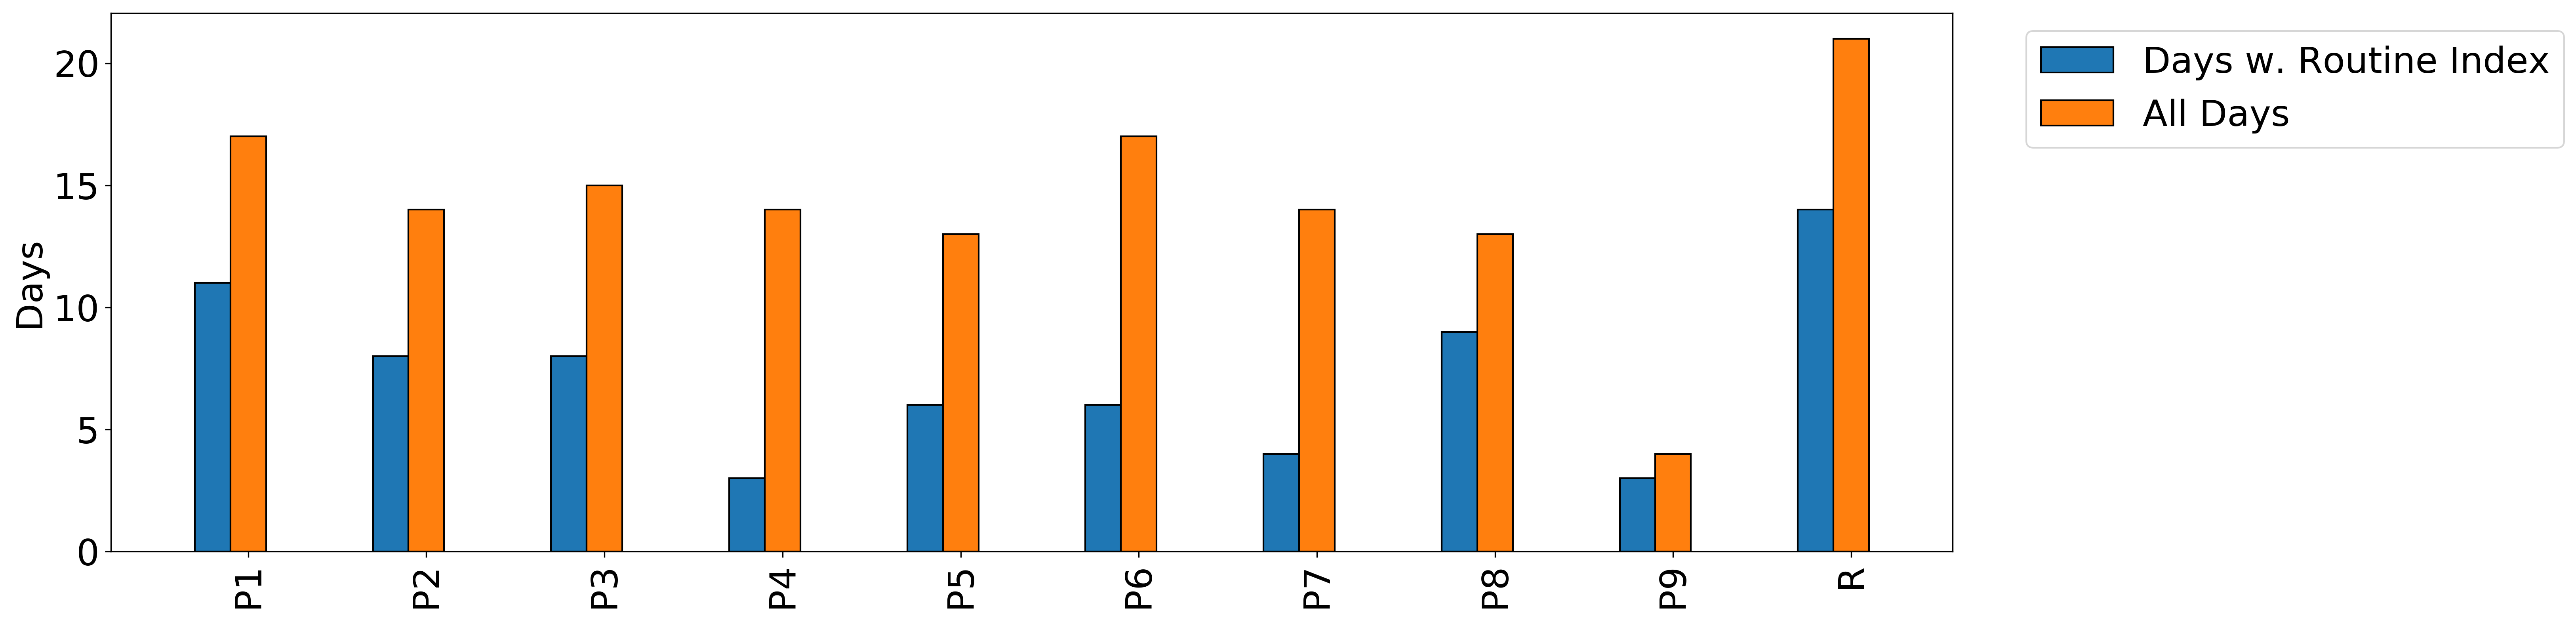
\includegraphics[width=\textwidth]{images/study/routine_valid_days.png}
    \caption{The days for which a given feature could be evaluated, out of the total days for which an answer was given and features were computed. As can be seen from the top plot, participant P4 had very few days where the home stay could be computed in comparison to the total number of days tracked which are above 20}
    \label{fig:plot-daily}
\end{figure}

The Home Stay feature is calculated by using the \textit{tracked} time at home, divided by the total time elapsed since midnight, and therefore a small gap in the data will make the feature undershoot. It is therefore to be expected that this feature will lie somewhat lower than the answer given by the user since there will be gaps in the data. 

\begin{figure}[h]
    \centering
    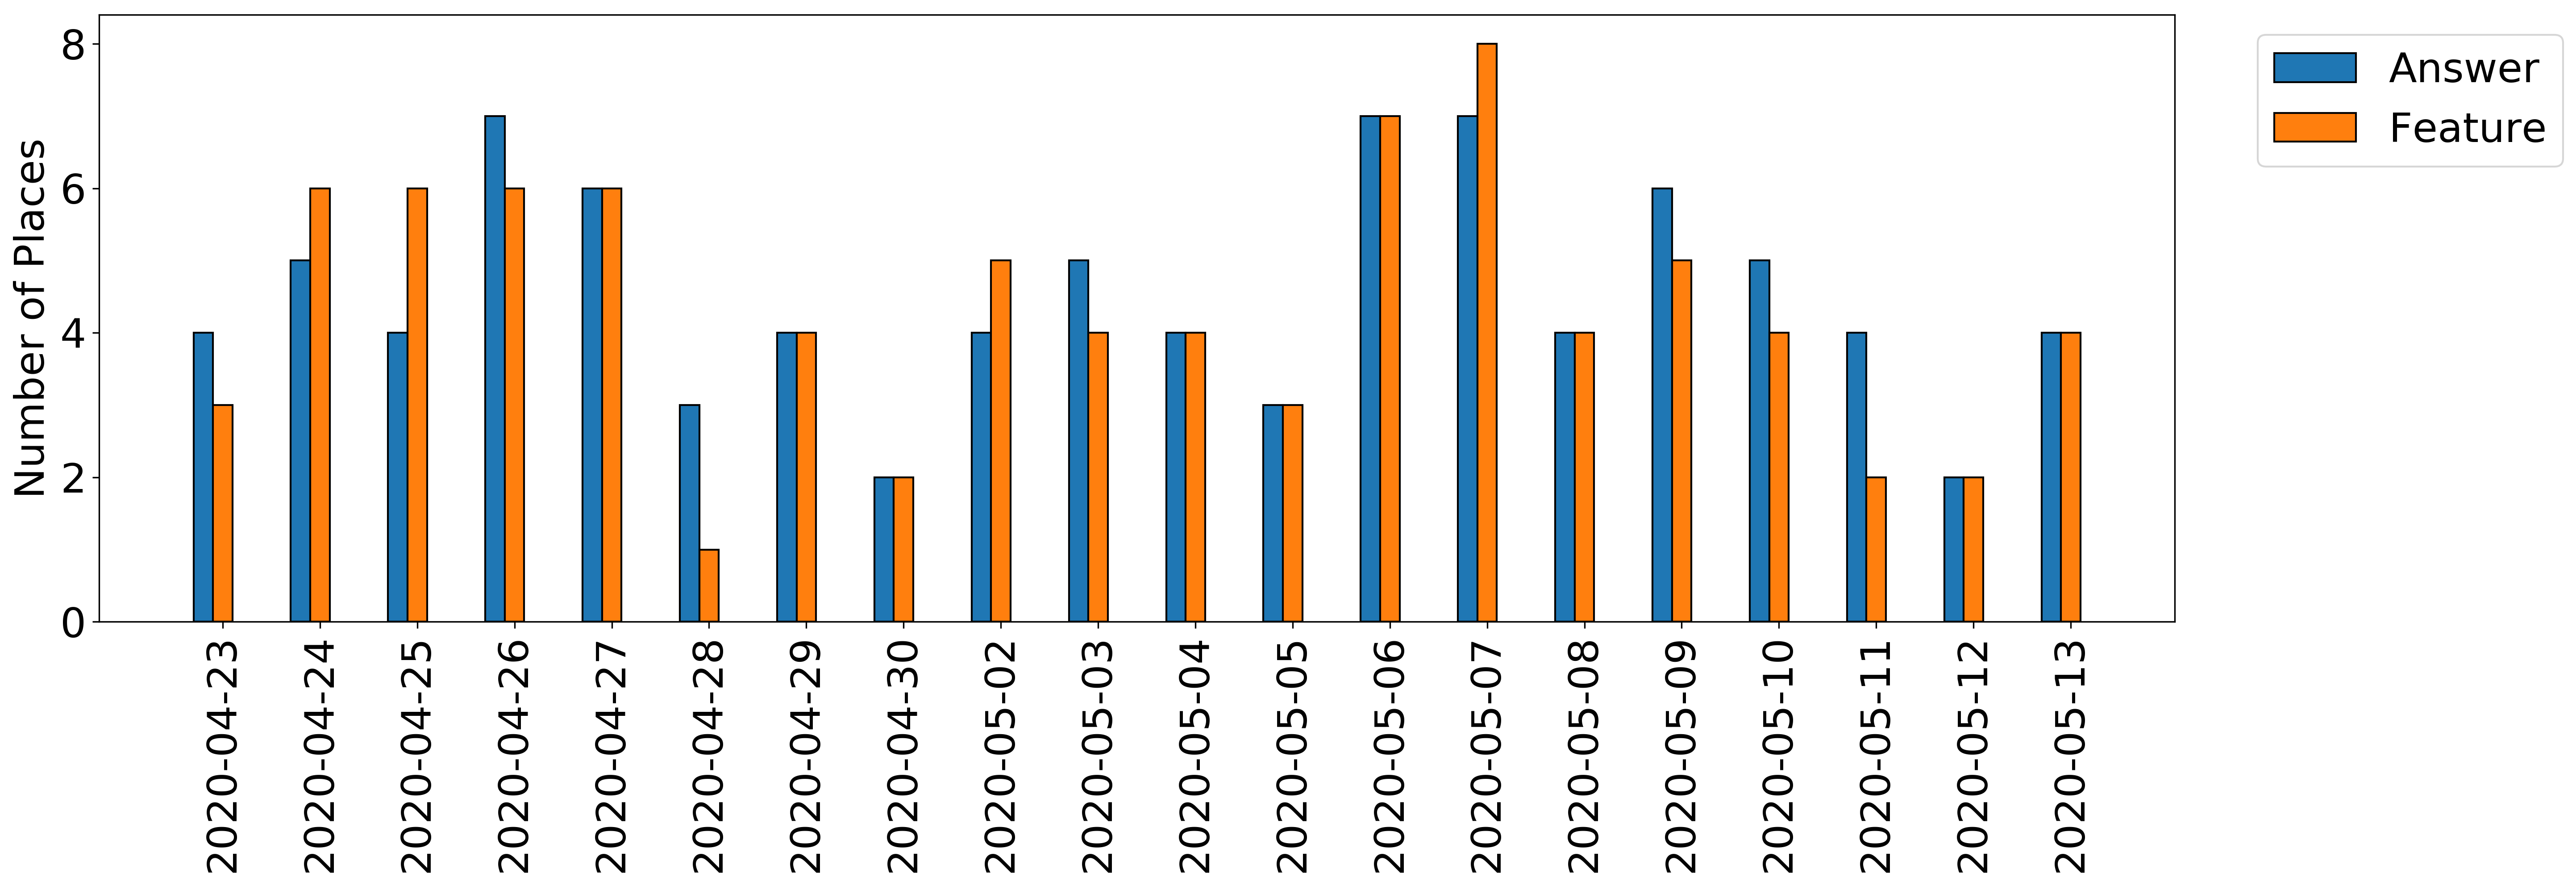
\includegraphics[width=\textwidth]{images/study/places_d6b2d9b9-398b-4e0d-b52b-224747f515c8.png}
    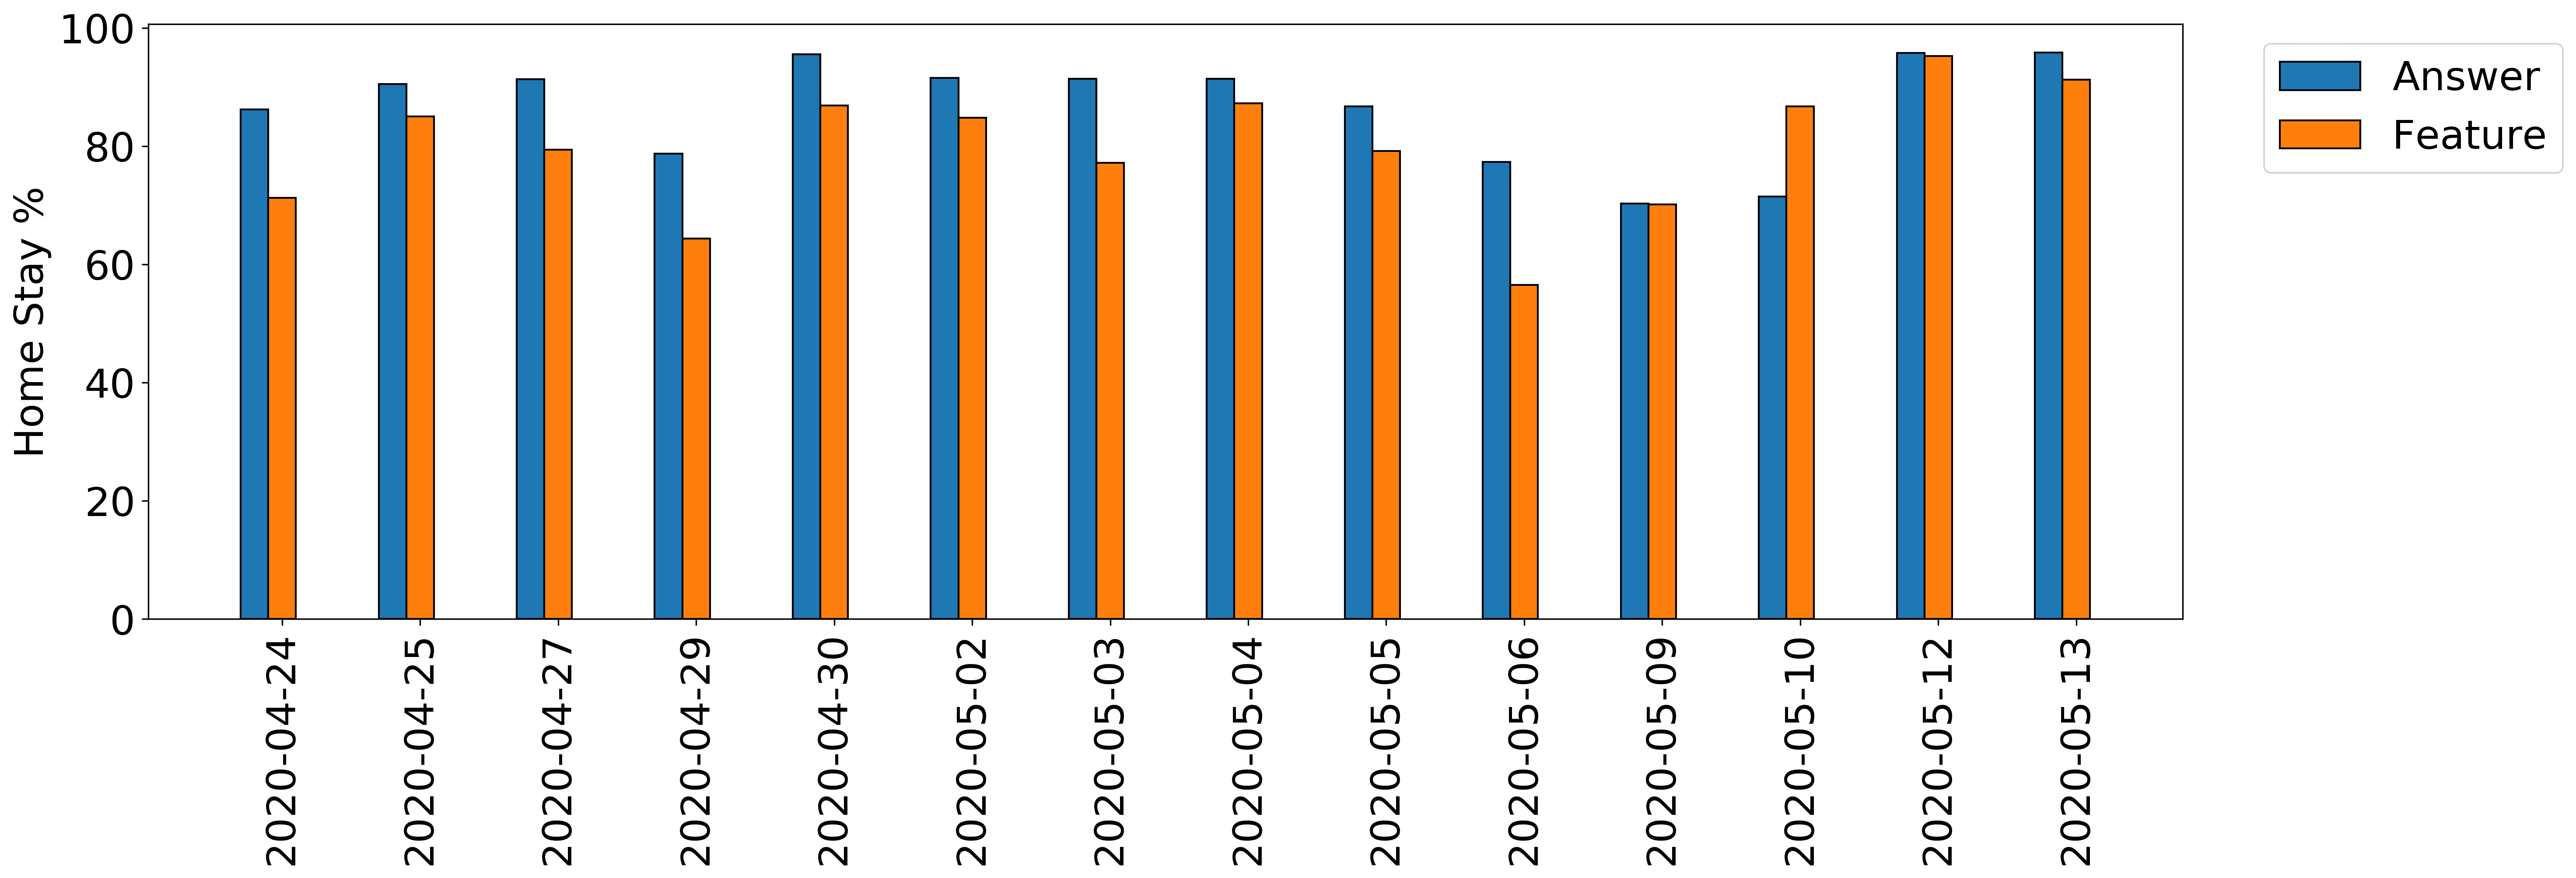
\includegraphics[width=\textwidth]{images/study/homestay_d6b2d9b9-398b-4e0d-b52b-224747f515c8.png}
    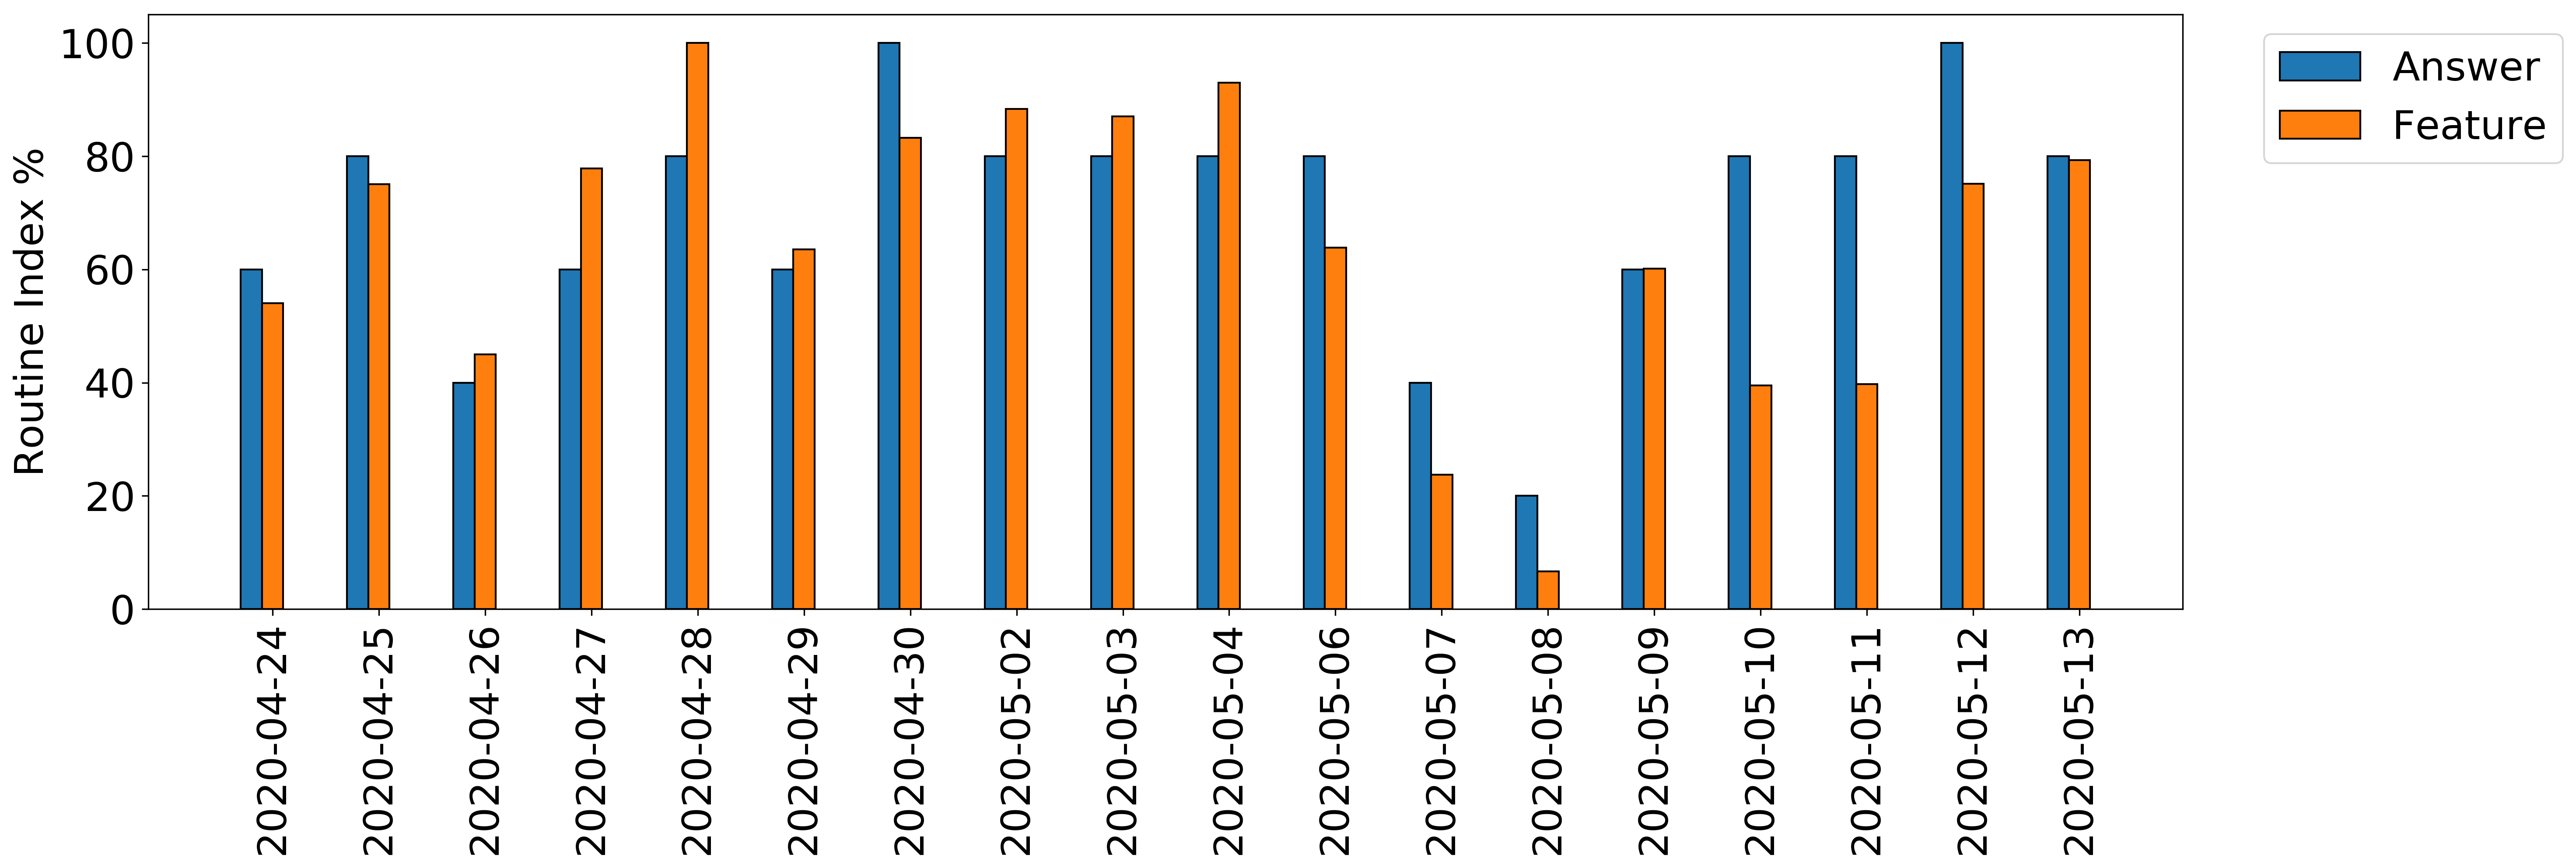
\includegraphics[width=\textwidth]{images/study/routine_d6b2d9b9-398b-4e0d-b52b-224747f515c8.png}
    \caption{The answered and calculated data for each day, for the author}
    \label{fig:plot-author-features}
\end{figure}

The day-by-day results for the author are displayed in figure \ref{fig:plot-daily} and from this plot, the computed features have a high correspondence with the provided answers. However, the feature computation is based on the author's own definitions which mean the computed features and answers of the author are also expected to be highly correlated. It is therefore relevant to show another participant, namely participant P8, who was very diligent in answering and tracking their location data. For this participant, very promising results were also produced which can be seen in Figure \ref{fig:plot-p8-features}.

\begin{figure}[h]
    \centering
    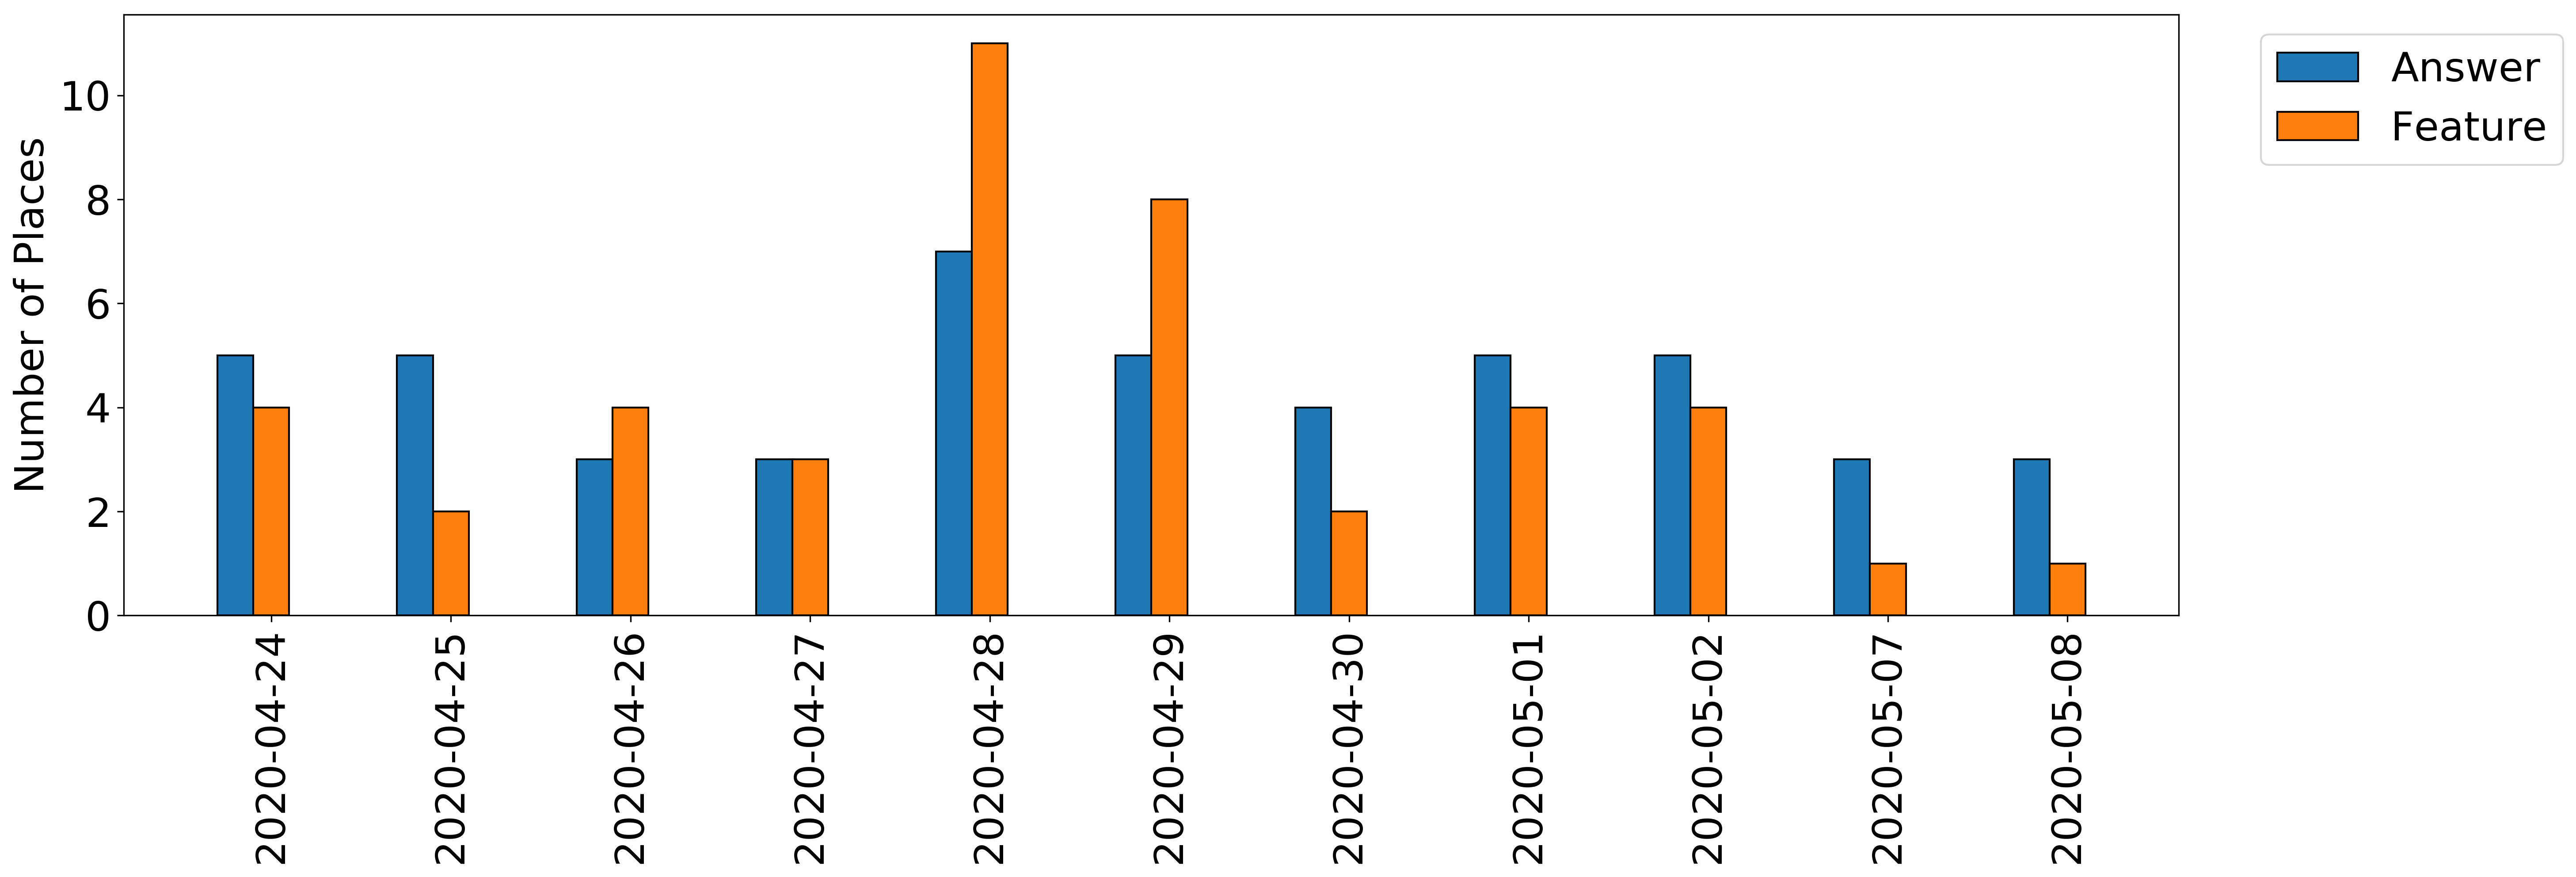
\includegraphics[width=\textwidth]{images/study/places_ec110976-0192-436d-b451-4f5dd97e71d8.png}
    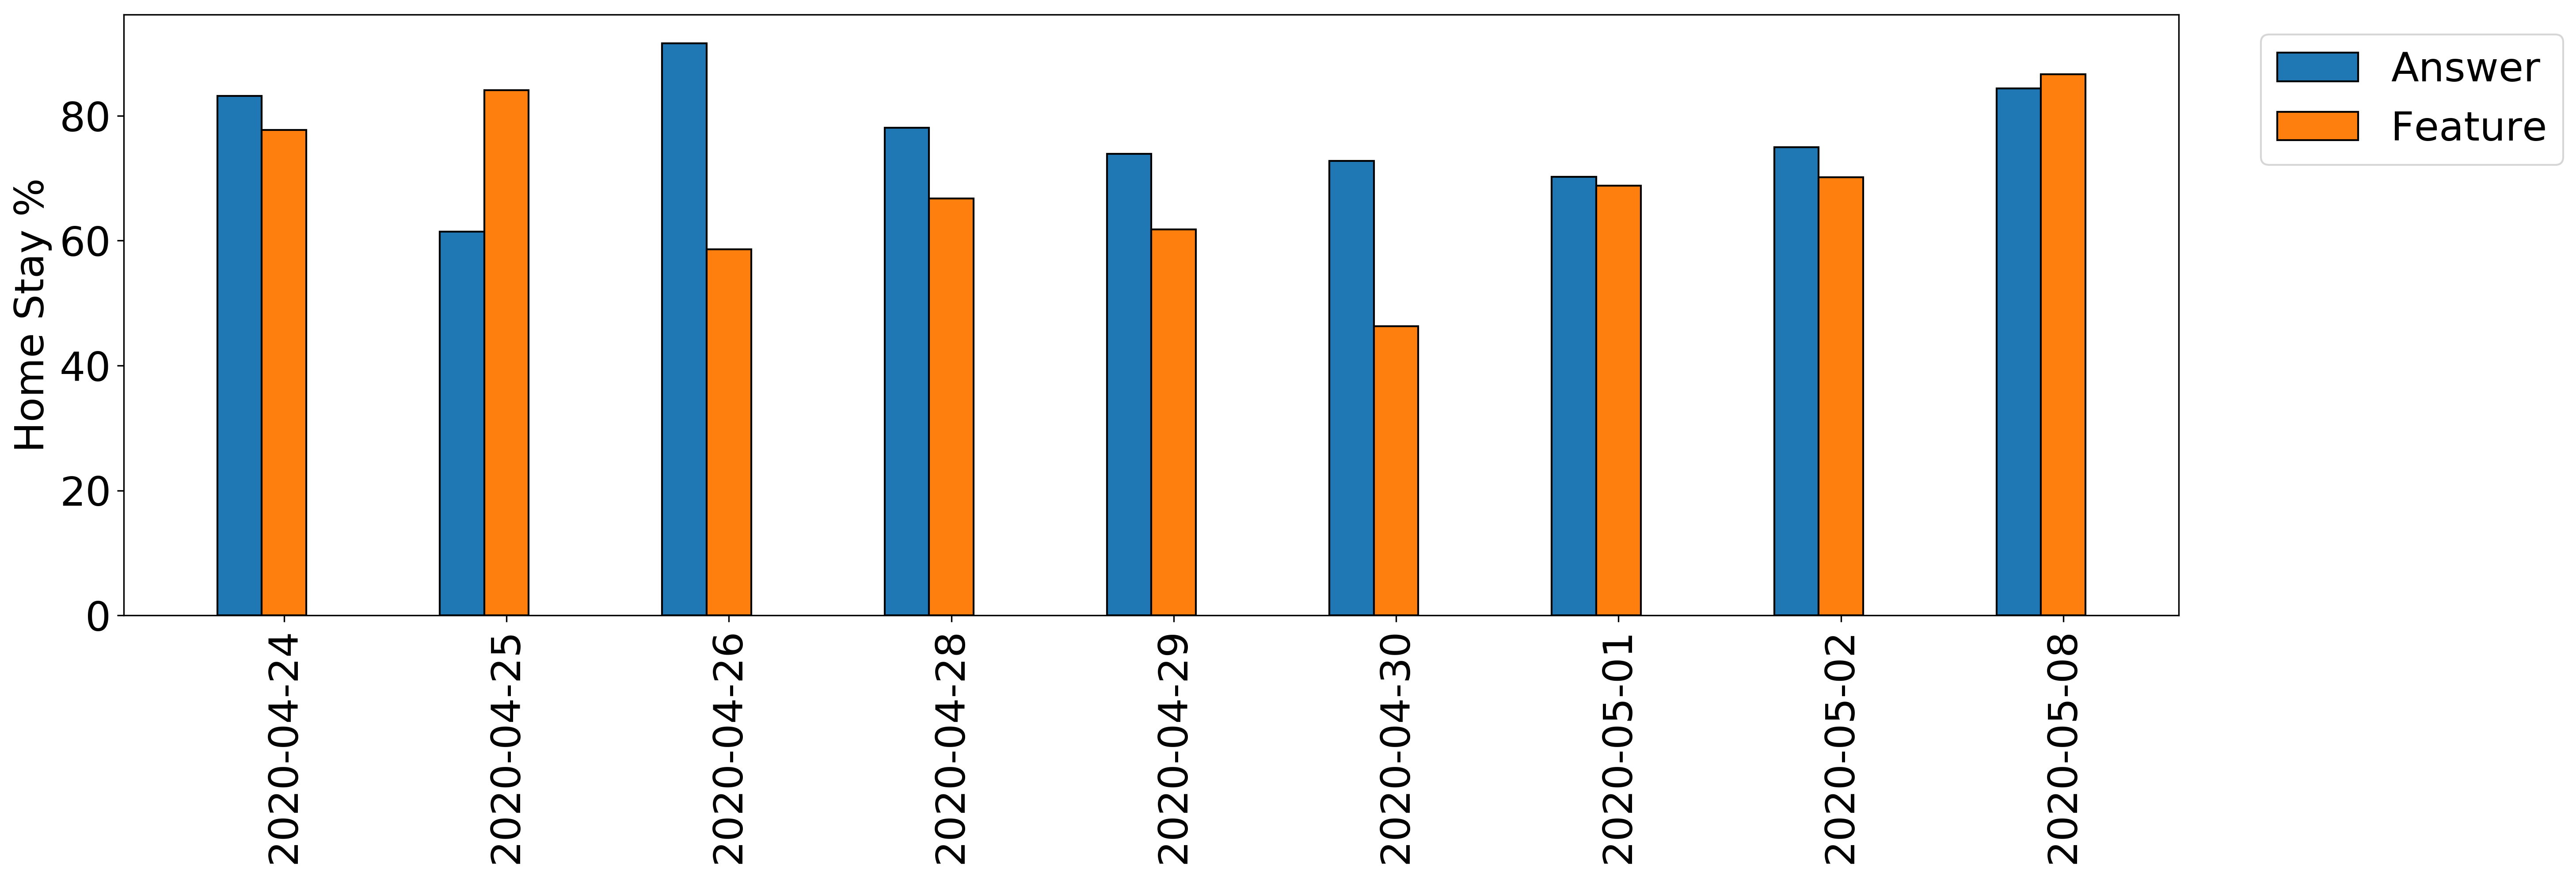
\includegraphics[width=\textwidth]{images/study/homestay_ec110976-0192-436d-b451-4f5dd97e71d8.png}
    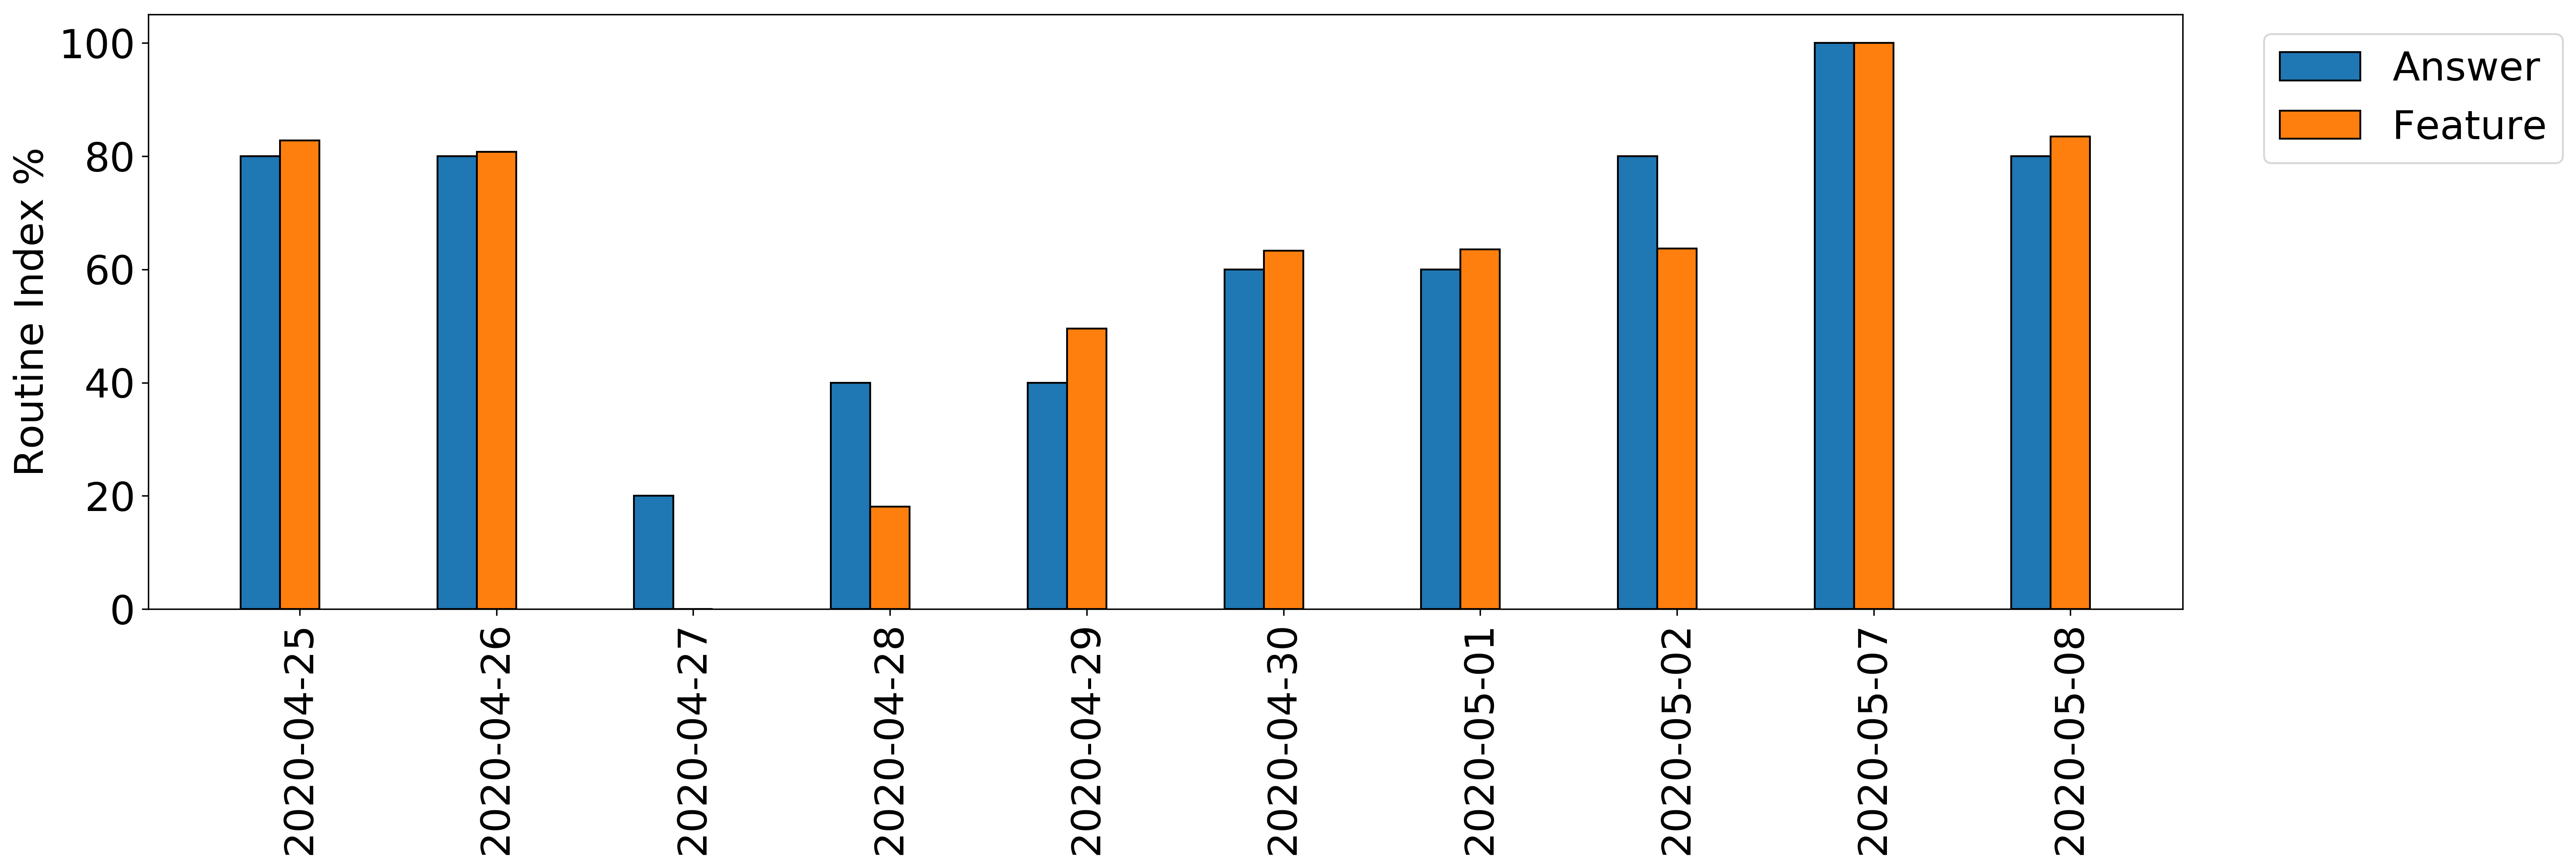
\includegraphics[width=\textwidth]{images/study/routine_ec110976-0192-436d-b451-4f5dd97e71d8.png}
    \caption{The answered and calculated data for each day for participant P8}
    \label{fig:plot-p8-features}
\end{figure}


\subsection{Measuring Errors}
There are a few ways data errors can occur:

\begin{itemize}
    \item The computed feature can be wrong due to gaps in the data (\textit{data collection error})
    \item The subjective answer from the user is wrong, e.g. if they misunderstood the concept of the question (\textit{answer error})
    \item Both of a \textit{data collection error} and an \textit{answer error} are made at the same time
\end{itemize}

Given this can occur, the RMSE was still computed for all three features across participants is shown in Table \ref{tab:error-table}. We observe the following:

\begin{itemize}
    \item The Number of Places predicted deviates with almost 1 place daily.

    \item The Home Stay percentage deviates with 14\% daily.

    \item The Routine Index deviates with 22.5\% daily. Here it is important to note than the Routine Index answer was given on scale with 20 percent increments which means that the 22.5\% RMSE is equivalent to one 'step' one the scale.
\end{itemize}

\begin{table}[]
    \centering
    \begin{tabular}{|l|l|l|l|}
    \hline
                        & \textbf{Number of Places} & \textbf{Home Stay} & \textbf{Routine Index} \\ \hline
    \textbf{Mean RMSE}       & 0.99                      & 14.27 (\%)         & 22.5 (\%)              \\ \hline
    \end{tabular}
    \caption{The mean RMSE computed for all participants}
    \label{tab:error-table}
\end{table}


To say something about whether or not the features undershoot or overshoot, the mean error was calculated for each participant as as $ME = \frac{\sum(F) - \sum(A)}{N}$ (where $N$ is the total number of days for the specific feature, for the participant). If the mean error is positive, the feature overshoots compared to the answered value, and vice versa if the error is negative. Since the mean error has a sign, i.e. either positive or negative, the 'mean' mean error cannot be computed. Instead, the individual mean error for each participant is plotted in Figure \ref{fig:plot-mean-error}. From this figure we observe the following:

\begin{itemize}
    \item The Number of Places feature undershoots by around 0.6 places or lower for most participants, with P7 being an outlier with -1.5 places. It is likely that the undershooting stems from \textit{data collection errors}, which can lead to places not being detected.

    \item The Home Stay feature undershoots for 8/10 participants, most of these having an error under 10\%. For those two participants where the feature overshoots, the error is also within 10\%. It is highly likely that the undershooting stems from \textit{data collection errors} leading to an underestimation of the time spent at home.

    \item The Routine Index feature is mixed with an equal number of participants for which it overshoots and undershoots. The current implementation of the feature will ignore time-slots for which data is missing, which leads to the Routine Index overshooting if a lot of data is missing. This feature is likely affected both by \textit{data collection errors} as well as \textit{answer errors}, hence the varying results.
\end{itemize}

\begin{figure}[h]
    \centering
    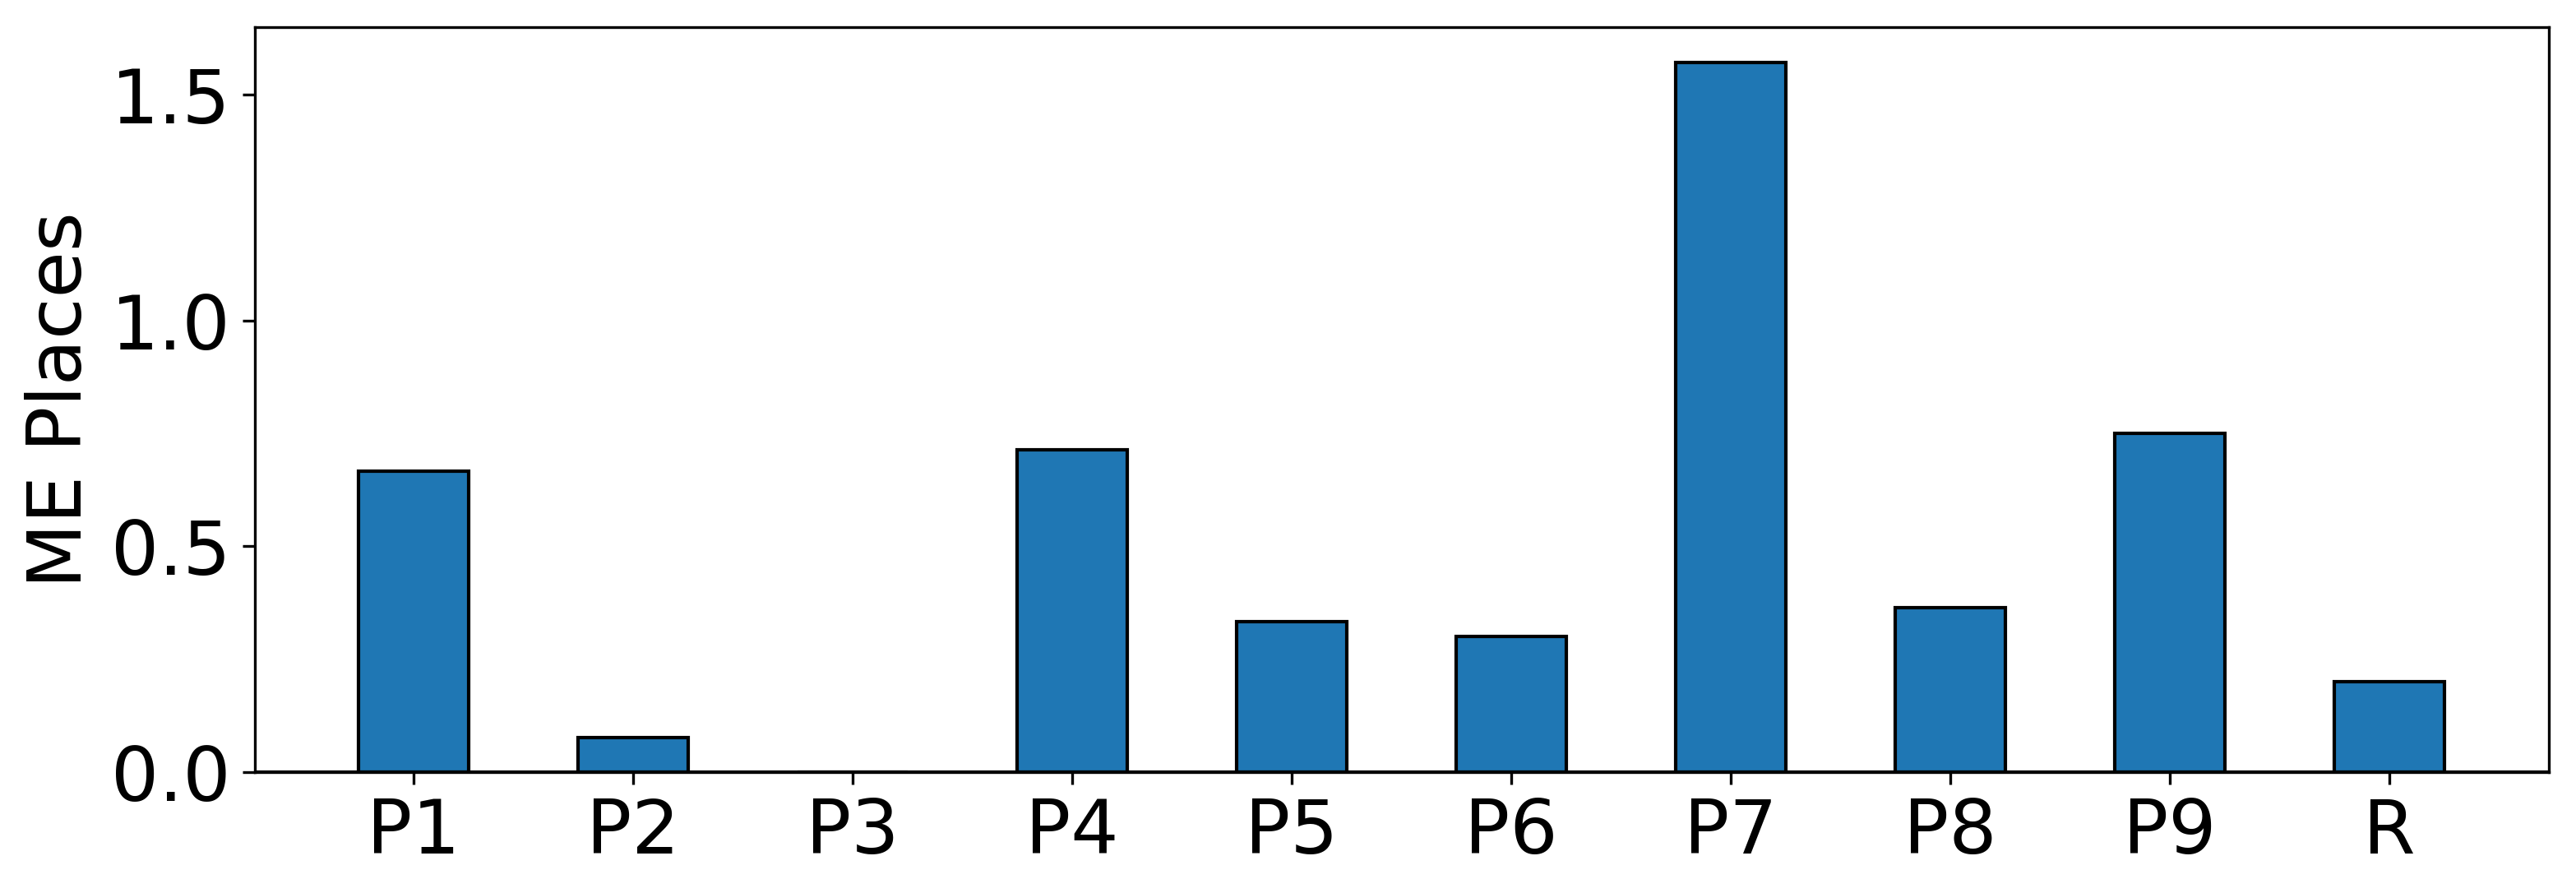
\includegraphics[width=\textwidth]{images/study/me_places.png}
    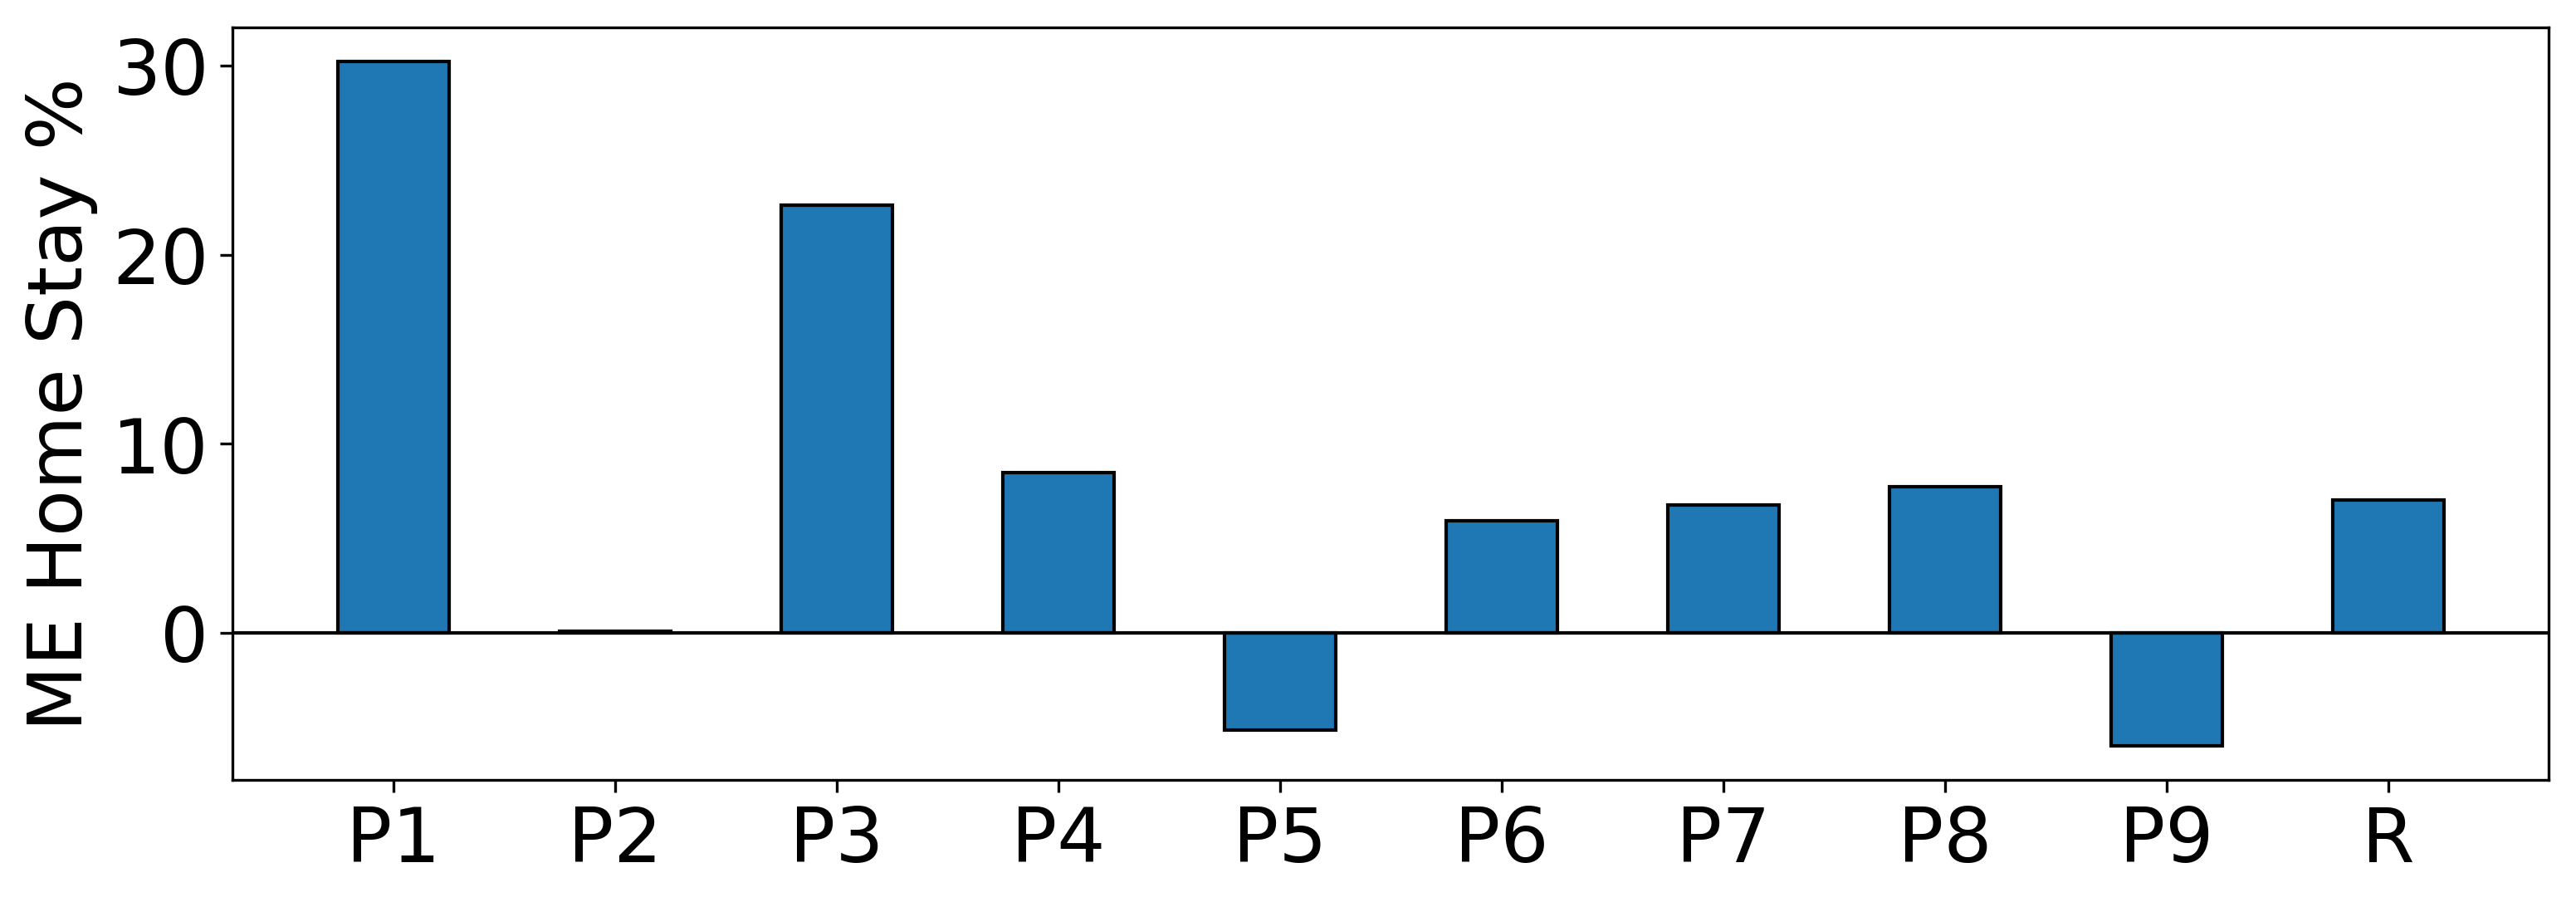
\includegraphics[width=\textwidth]{images/study/me_homestay.png}
    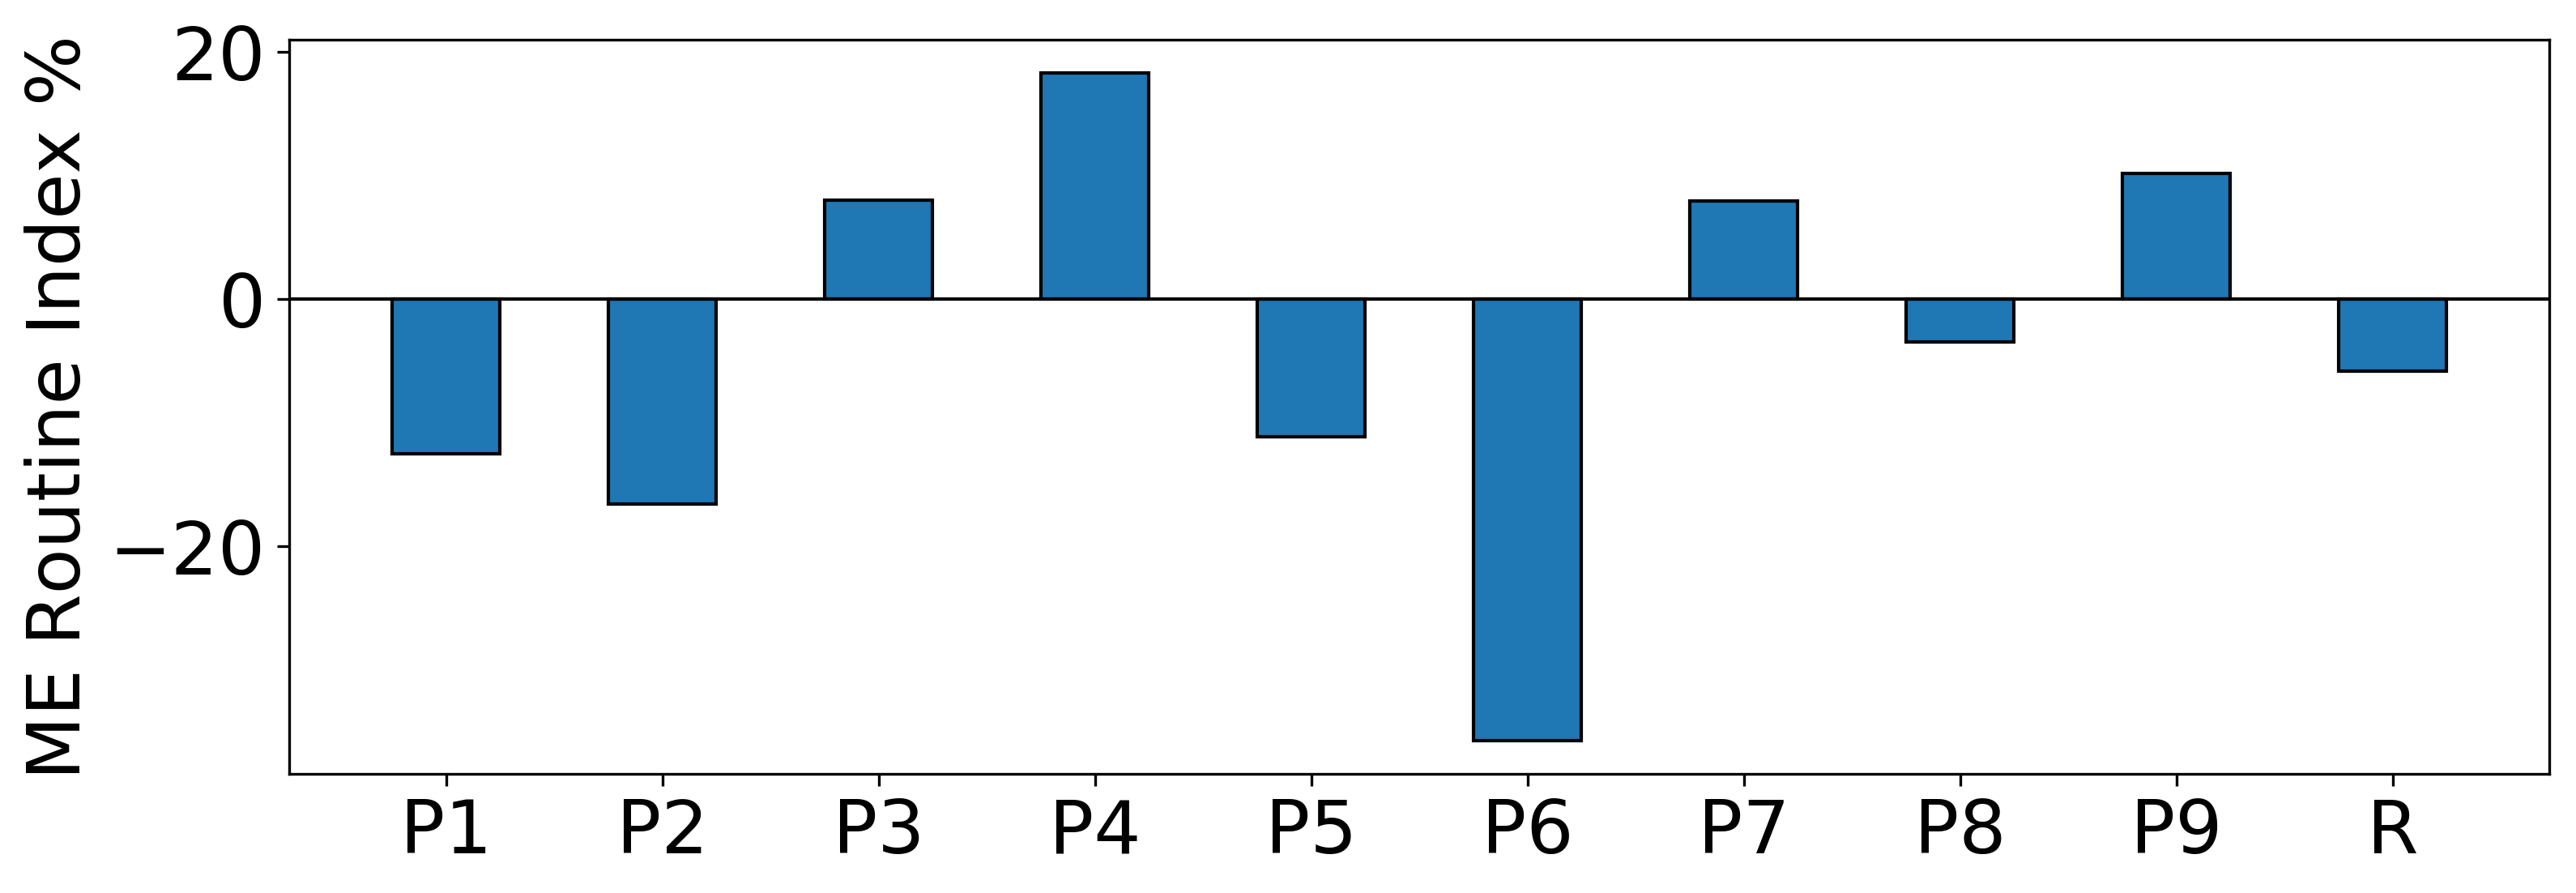
\includegraphics[width=\textwidth]{images/study/me_routine.png}
    \caption{The mean error for each participant for each of the three features. A negative mean error means the computed feature undershoots, and a positive error means it overshoots}
    \label{fig:plot-mean-error}
\end{figure}




\section{Improvements}
Now we have a data set with measurements and 'ground truth'
parameter tuning
Look for knee on the graph, aim for lowest generalization error
Machine learning task

\section{Privacy}

\section{Package Limitations}
Not so easy to use right now
Many lines of code
Manual saving data
In the end this will be automatically done

\section{Maintenance}
It will be a real package, which will be maintained

\section{Results}

\section{Future Work}
Integrating this into apps people already\\
Give concrete recommendations, ex Rohani MUBS\\

\section{User Prompting in Real-Time}
When should the user be given recommendations\\
Trigger can be time interval or threshold for a feature, i.e. if homestay greater than 0.5 prompt the user to leave the house\\
Recommendations from depression database (Rohani, 300 items, not part of this thesis)\\

Calculate routine index from week to week rather than day to day. Currently we assume that all days ideally look identical, which for most people will not be the case. For many people the weekends differ quite a lot from their every day, and naturally the routine index will therefore be lower during the weekend, and weekend days will tend to 'wash out' the routine index calculation. 

\section{Calculations}
\subsection{Home Stay}
It was found that the total time spent at stops was sometimes differing from the  total amount of time in a day, i.e. 24 hours, and was often quite a bit lower. This meant the proposed home stay would be quite high. There were three different approached considered, which where to sum the total amount of time spent at stops on the day, consider the total to be the difference between the arrival at the first stop and departure from the last stop, or lastly to simply let it be defined as the amount of time of day, i.e. the home stay calculated at 13:30 would consider the total to be 13.5 hours.  